% \section{Relative weights accuracy}

% \section{Posterior distributions compared to proportion of variance explained}

% I picture running a linear regression model with different correlation values for two, three and maybe 4 covariates and discuss the effects of this.

% \subsection{Linear regression}
% \subsubsection{Analytical solutions}
% \subsubsection{Impact of correlated data}

% \subsection{Linear regression with a random intercept}

% \subsection{Linear regression with two or more random intercept}

% \subsection{LMM's?}

% \subsection{Analytical solutions(if included)}

% \section{Interpretations, findings and $R^2$}
\section{Insights from the simulation study}
To present the results of the simulation study we consider each effect separately in different plots, that is we show results for the importance of variables $X_1, X_2, X_3$ and the random effect $\boldsymbol{\alpha}$, in distinct plots. 
We used violin plots to visualize the estimated quantities, as they contain much information in a compact way. The violin plot is analogous to a density plot, but the density is shown along the $y$-axis and mirrored about the $y$-axis to form a symmetrical shape. Each violin therefore displays the distribution of our simulated estimates.
Lastly, we consider how our BVI model estimates the conditional and marginal $R^2$ values from a Bayesian perspective, comparing these results to the $R^2$ value obtained from the decompositions by the Relaimpo, ELMG, and ERW methods, where the first method only considers models without random effects. 
\subsection{Relative importance of the fixed effects}
\label{sec:relimp_fixed}
In \Cref{fig:relimp_X1,fig:relimp_X2,fig:relimp_X3} the distribution of the relative importance allocated to each fixed effect from the simulations are shown.
There are four different distributions for each method, which corresponds to the four different correlation levels. 
The horizontal dashed line displays the theoretically correct relative importance when the covariates are pairwise independent. 
\newline
\newline
In general, it can be seen that the distributions in the case of uncorrelated data are unbiased with some variation around the theoretically correct relative importance.
For a correlation of $\rho=0.1$ the distributions of the estimates are shifted marginally compared to the uncorrelated case for all methods.
The importance attributed to $X_1$ and $X_2$, in \Cref{fig:relimp_X1}a and \Cref{fig:relimp_X2}b respectively, is larger when compared to the uncorrelated case, whereas the importance attributed to $X_3$ in \Cref{fig:relimp_X3}c is smaller.
All methods seem to shift the relative importance estimate for the covariate with the same amount in the same direction.
This shift is both expected and desirable, when considering the values found in \Cref{table:1} for the theoretically correct variance explained. 
Therefore, we should expect our method to assign different shares when we have various levels of covariate correlation, which it does.
This trend continues for the correlation level $\rho=0.5$, where the distributions are shifted further in the same directions as for $\rho=0.1$.
Lastly, for $\rho=0.9$ we see the largest reallocation of the distributions, which follows the same trend as for the other correlation levels.
\newline
\newline
The rise in importance for $X_1$ and $X_2$ for increasing correlation can be understood by the relation $\mathbf{Z}\boldsymbol{\Lambda}=\mathbf{X}$ in the relative weights method. 
When the matrix $\mathbf{X}$ is not correlated, $\boldsymbol{\Lambda}$ is close to the identity matrix, but with an increase in correlation the diagonal elements grows smaller and off diagonal elements grow larger.
An increase in off diagonal values would for $X_1$ and $X_2$ imply that a larger value is multiplied with $\beta_3^2$, which is larger than $\beta_1^2$ and $\beta_2^2$. 
Therefore, it is expected to see a rise in importance as correlation increases for $X_1$ and $X_2$, and the opposite for $X_3$.
In all figures, the BVI method is in agreement with the other methods when allocating importance for different correlation levels.
The width of the distributions seem to become lower as the correlation increases, most notably for $\rho=0.9$, where the distributions exhibit significantly smaller dispersion than for $\rho=0$.
Generally all methods seem to follow the same trends and produce similar results for all three fixed effects. 
As correlation increases the trend is that the relative importance assigned to $X_1$ and $X_2$ increases, in contrast to the decrease in relative importance assigned to $X_3$.
\newline
\newline
In general, the BVI method is in agreement with the theoretical results for uncorrelated data derived in \Cref{ch:method} and is consistent with the other three methods for correlated fixed effects. 
\begin{figure}[H]
  \centering
    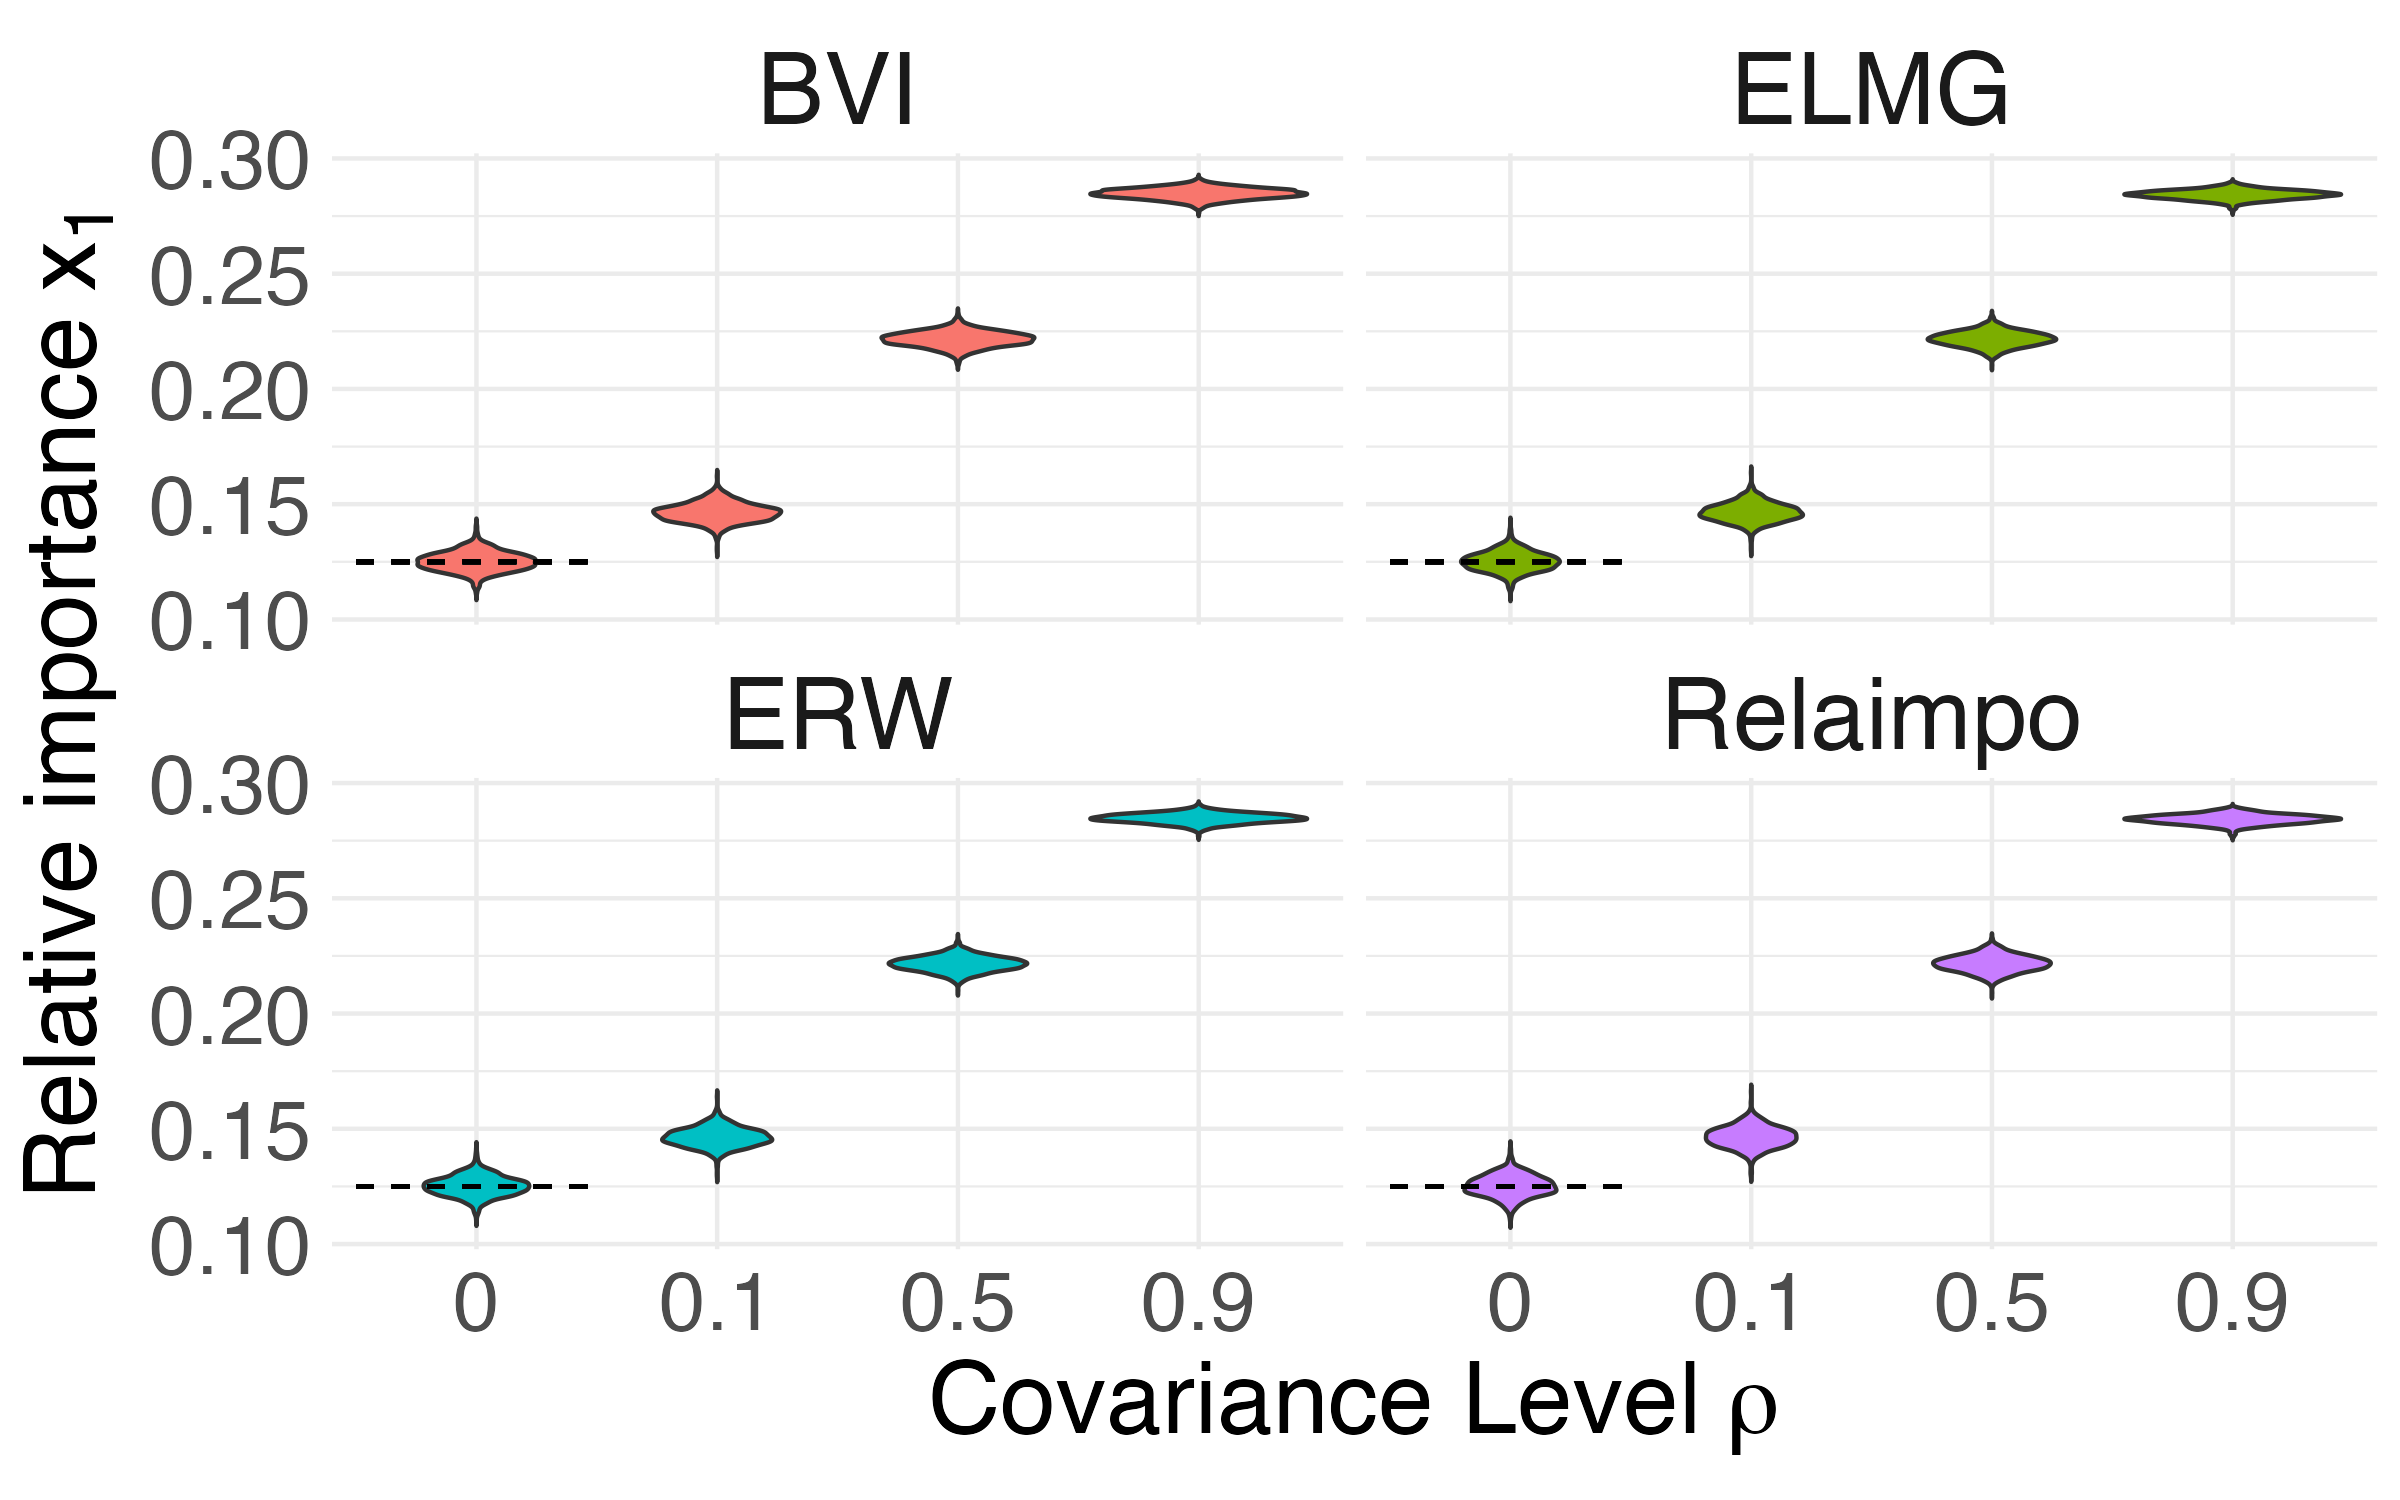
\includegraphics[width=0.7\linewidth]{Figures/ViolinPlots/Variance_V1.png}
    \caption{Violin plots for the relative importance of the fixed effects $X_1, X_2$ and $X_3$ for different correlation levels calculated from the ensemble of simulated datasets by the BVI, ELMG, ERW and the Relaimpo methods. The standardized regressor coefficients are $\boldsymbol{\beta}=\left(\sqrt{1/8}, \sqrt{2/8}, \sqrt{3/8}\right)$, and the true total model variance is $\sigma^2_{\mathbf{y}}=1$. For the BVI method the distributions of posterior means are shown to compare to the distribution of point estimates from the other three methods. The horizontal line displays the theoretically correct importance of each fixed effect in the case of uncorrelated data. (a) Relative importance of $X_1$ as calculated from the four methods.}
    \label{fig:relimp_X1}
\end{figure}
\begin{figure}[H]\ContinuedFloat
  \centering
    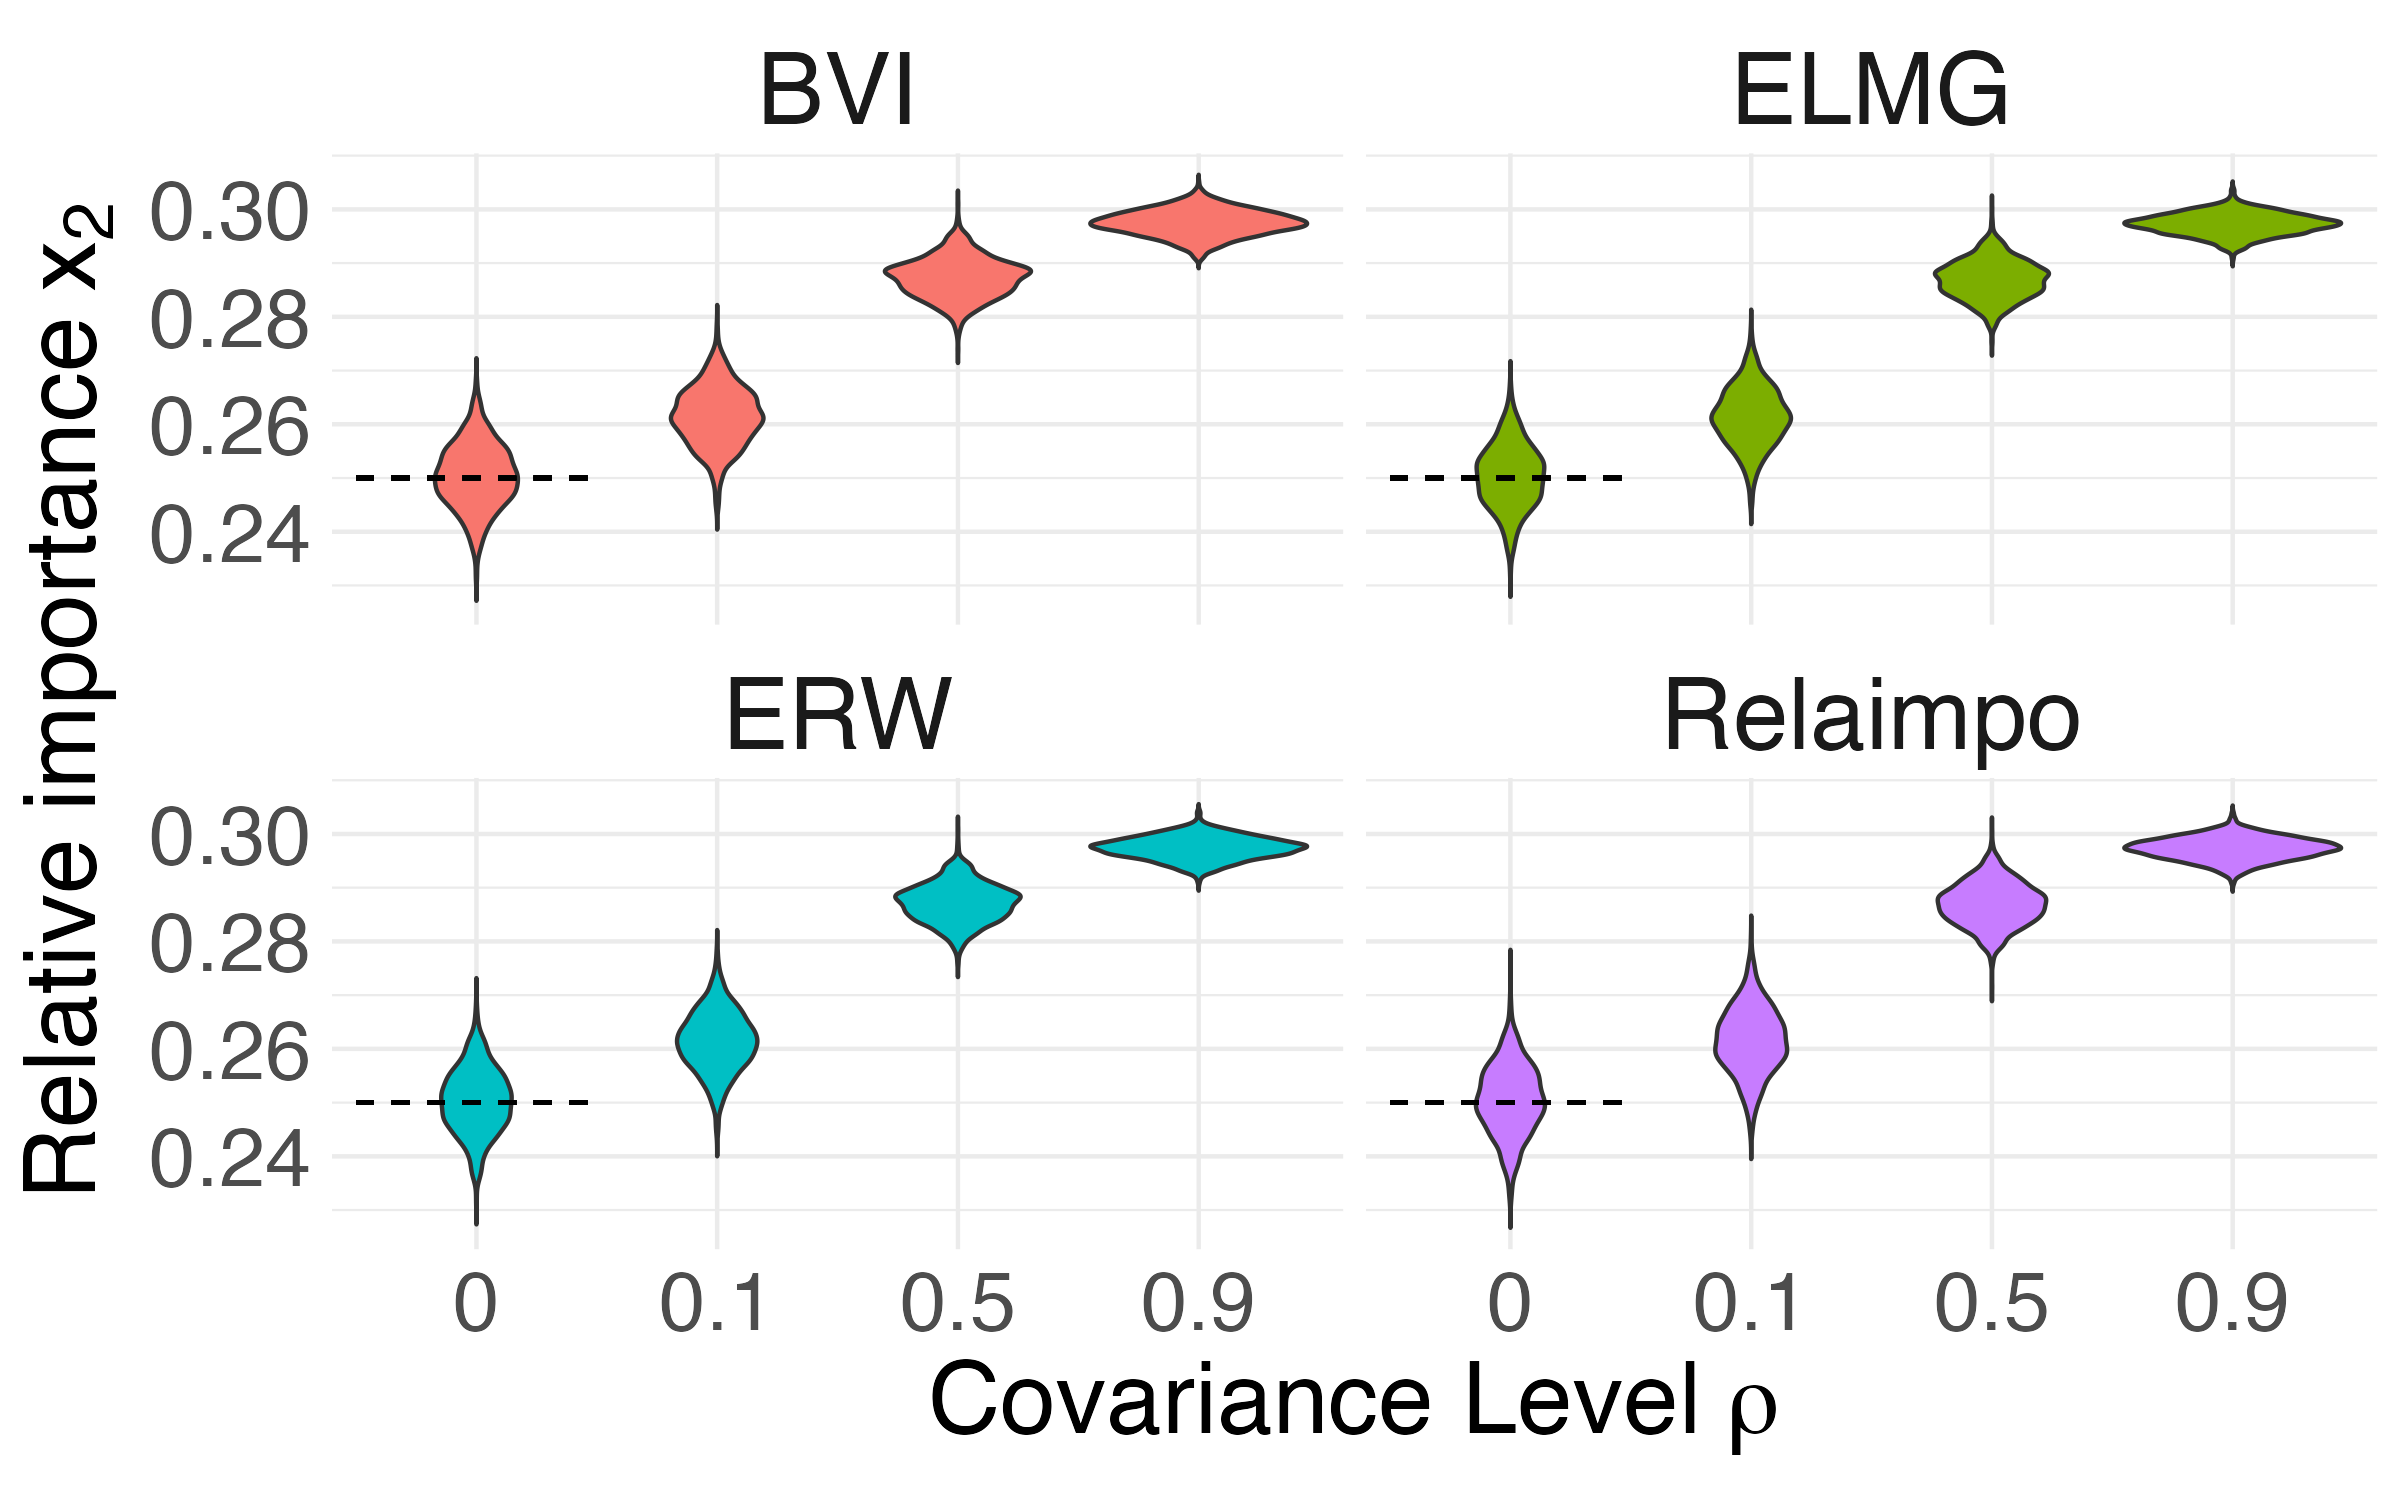
\includegraphics[width=0.7\linewidth]{Figures/ViolinPlots/Variance_V2.png}
    \caption{(b) Relative importance of $X_2$ as calculated from the four methods.}
    \label{fig:relimp_X2}
\end{figure}
\begin{figure}[H]\ContinuedFloat
  \centering
    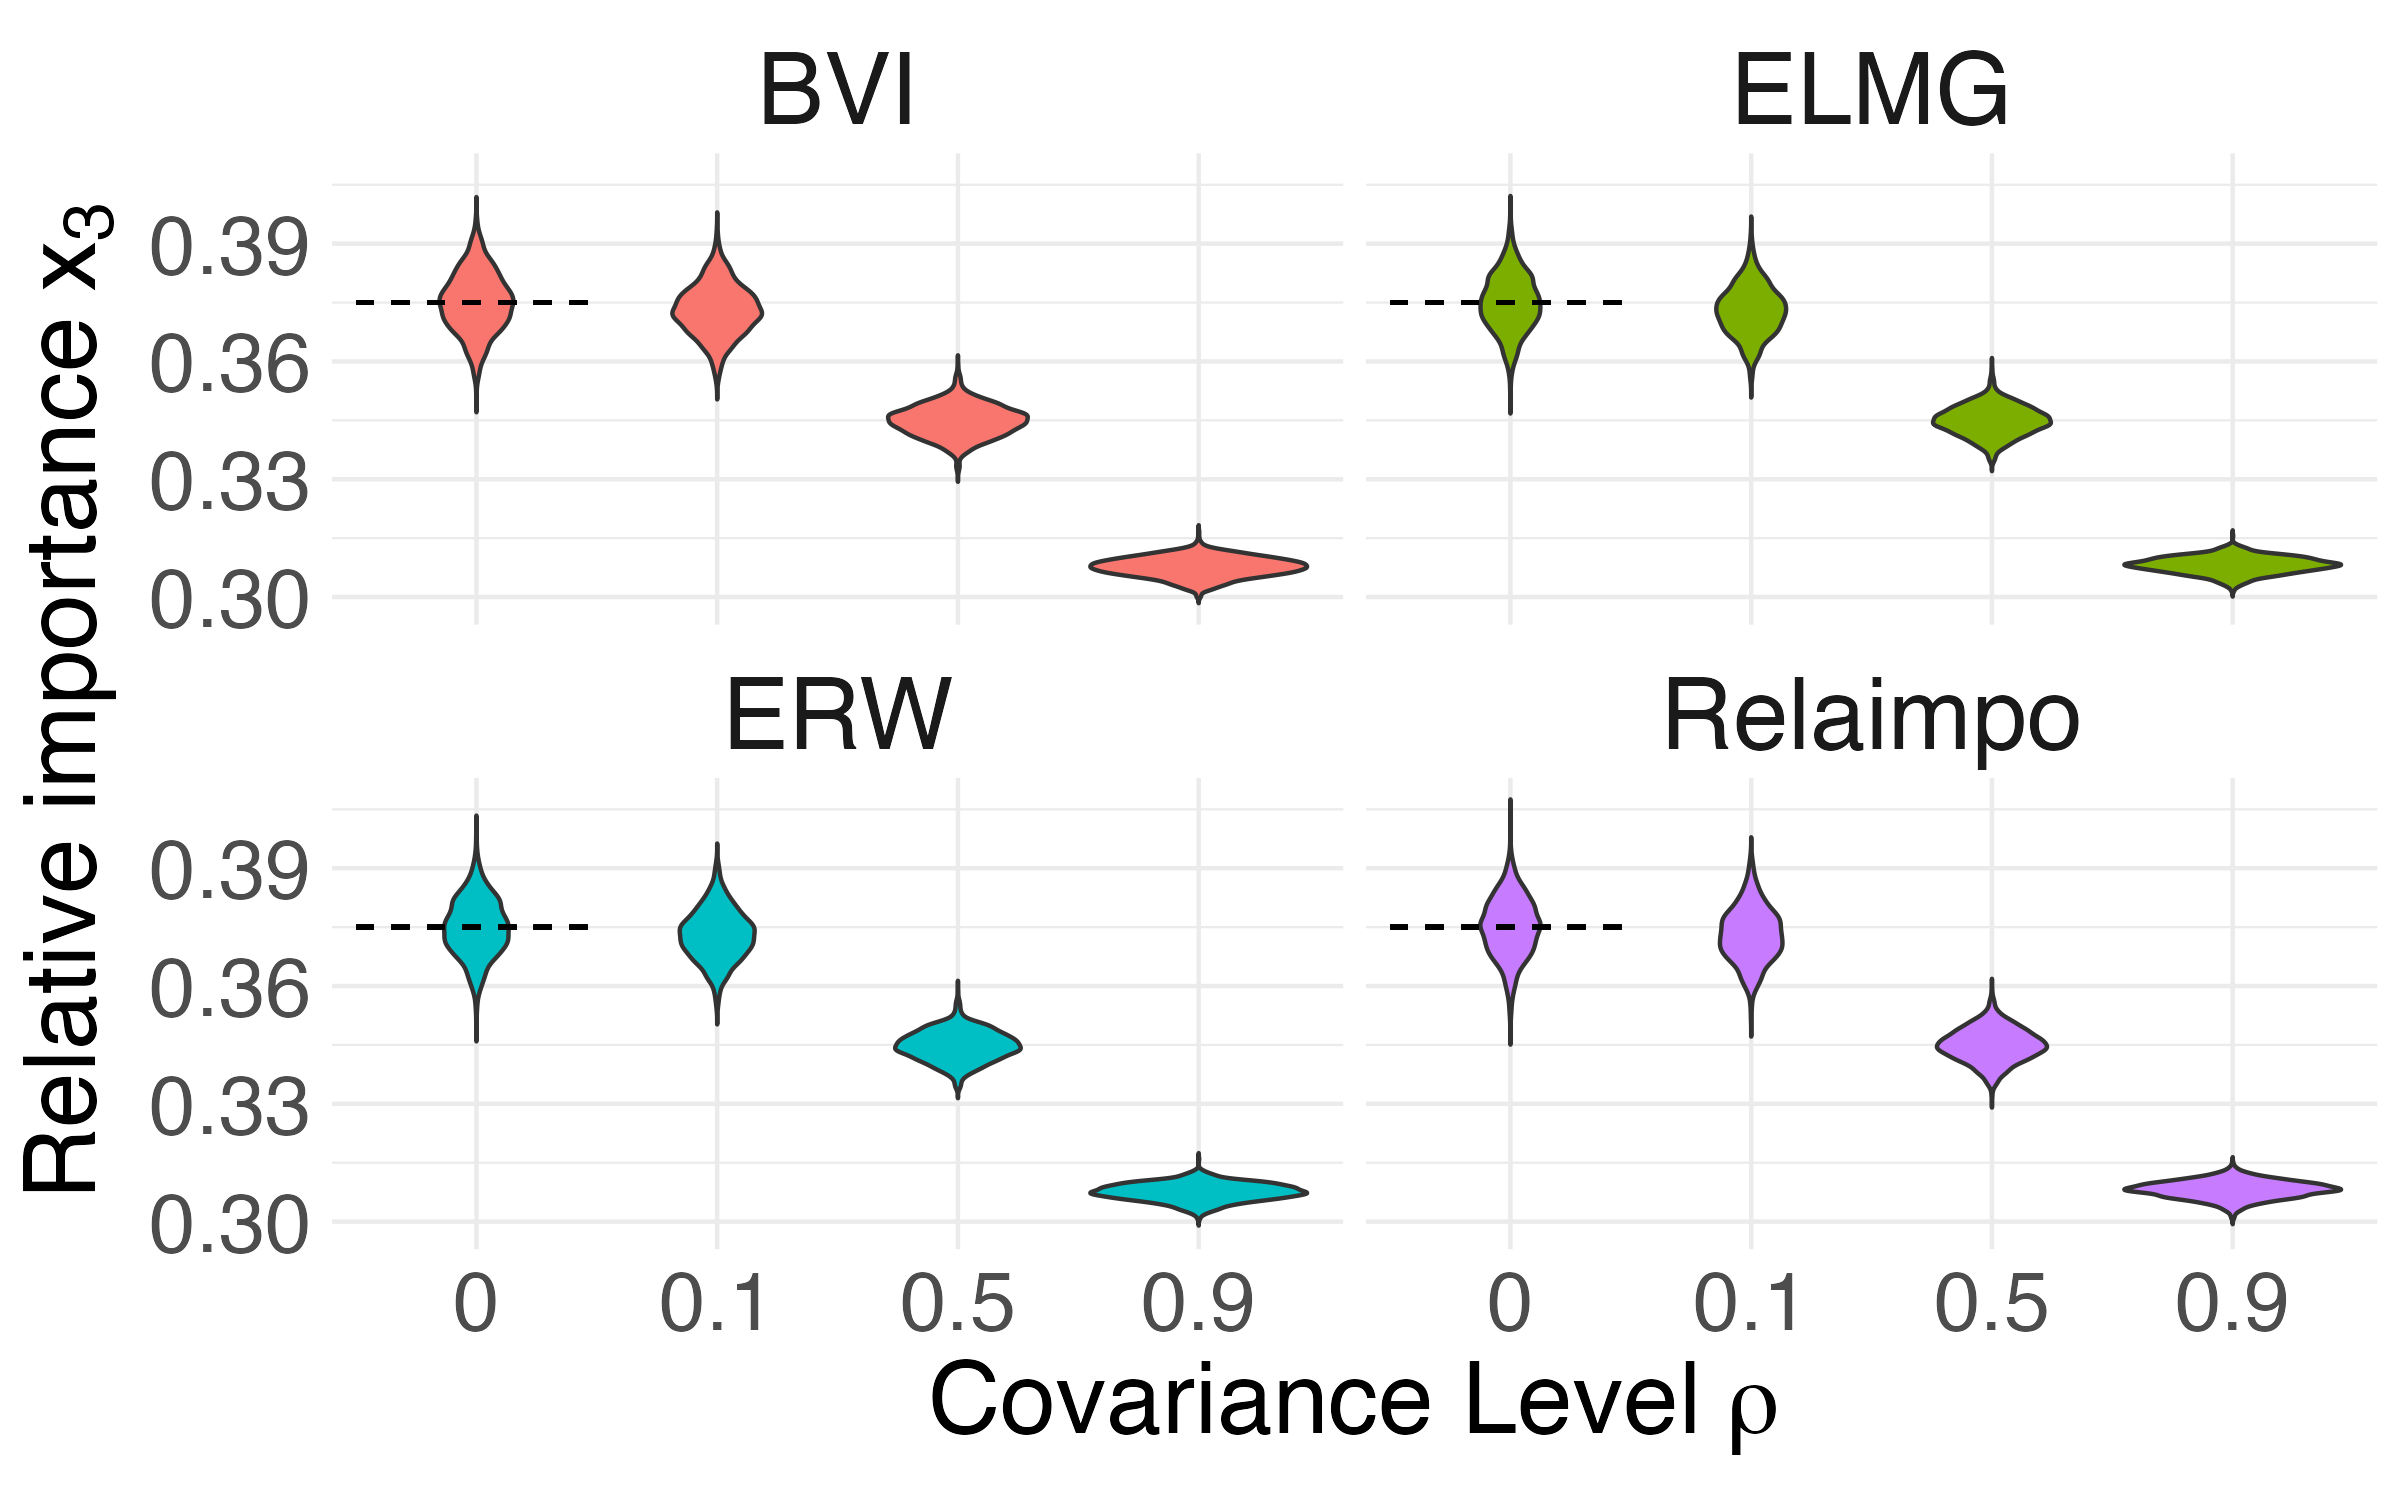
\includegraphics[width=0.7\linewidth]{Figures/ViolinPlots/Variance_V3.png}
    \caption{(c) Relative importance of $X_3$ as calculated from the four methods.}
    \label{fig:relimp_X3}
\end{figure}


% \begin{figure}[H]
%   \centering
%   \subfloat[Relative importance of $X_1$ as calculated from the four methods.]{
%     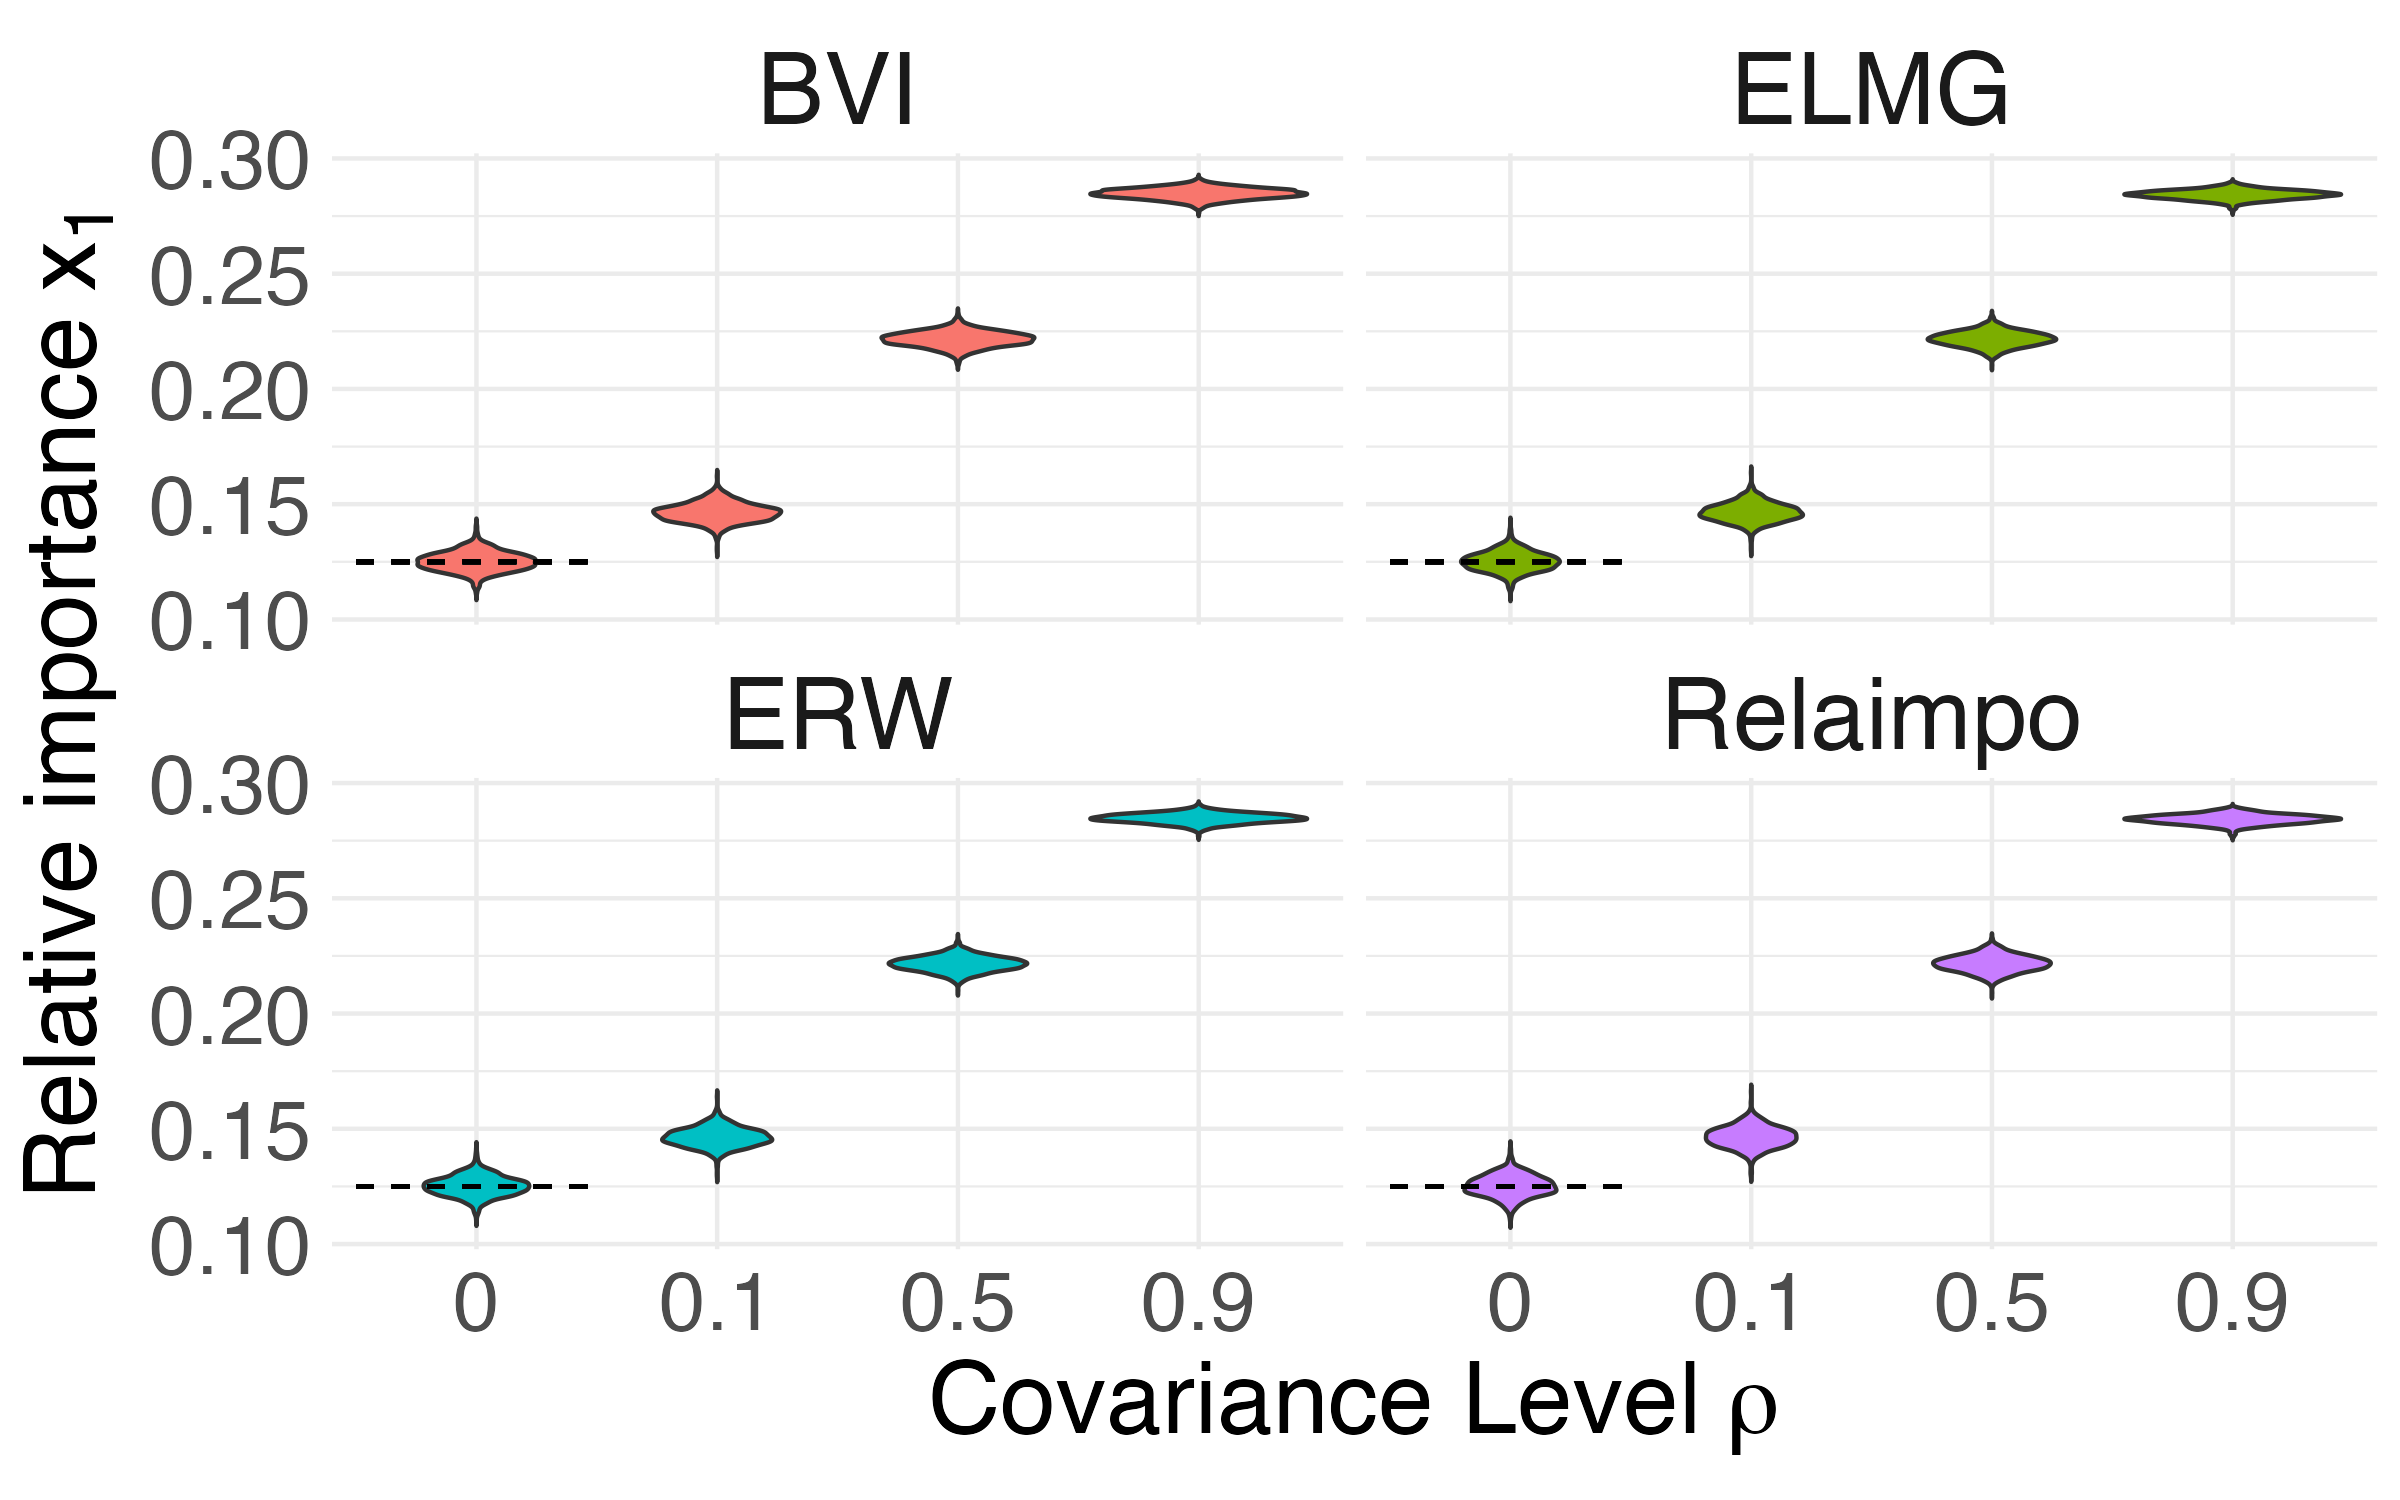
\includegraphics[width=0.6\linewidth]{Figures/ViolinPlots/Variance_V1.png}
%     \label{fig:relimp_X1}
%   }
%   \hfill
%   \subfloat[Relative importance of $X_2$ as calculated from the four methods.]{
%     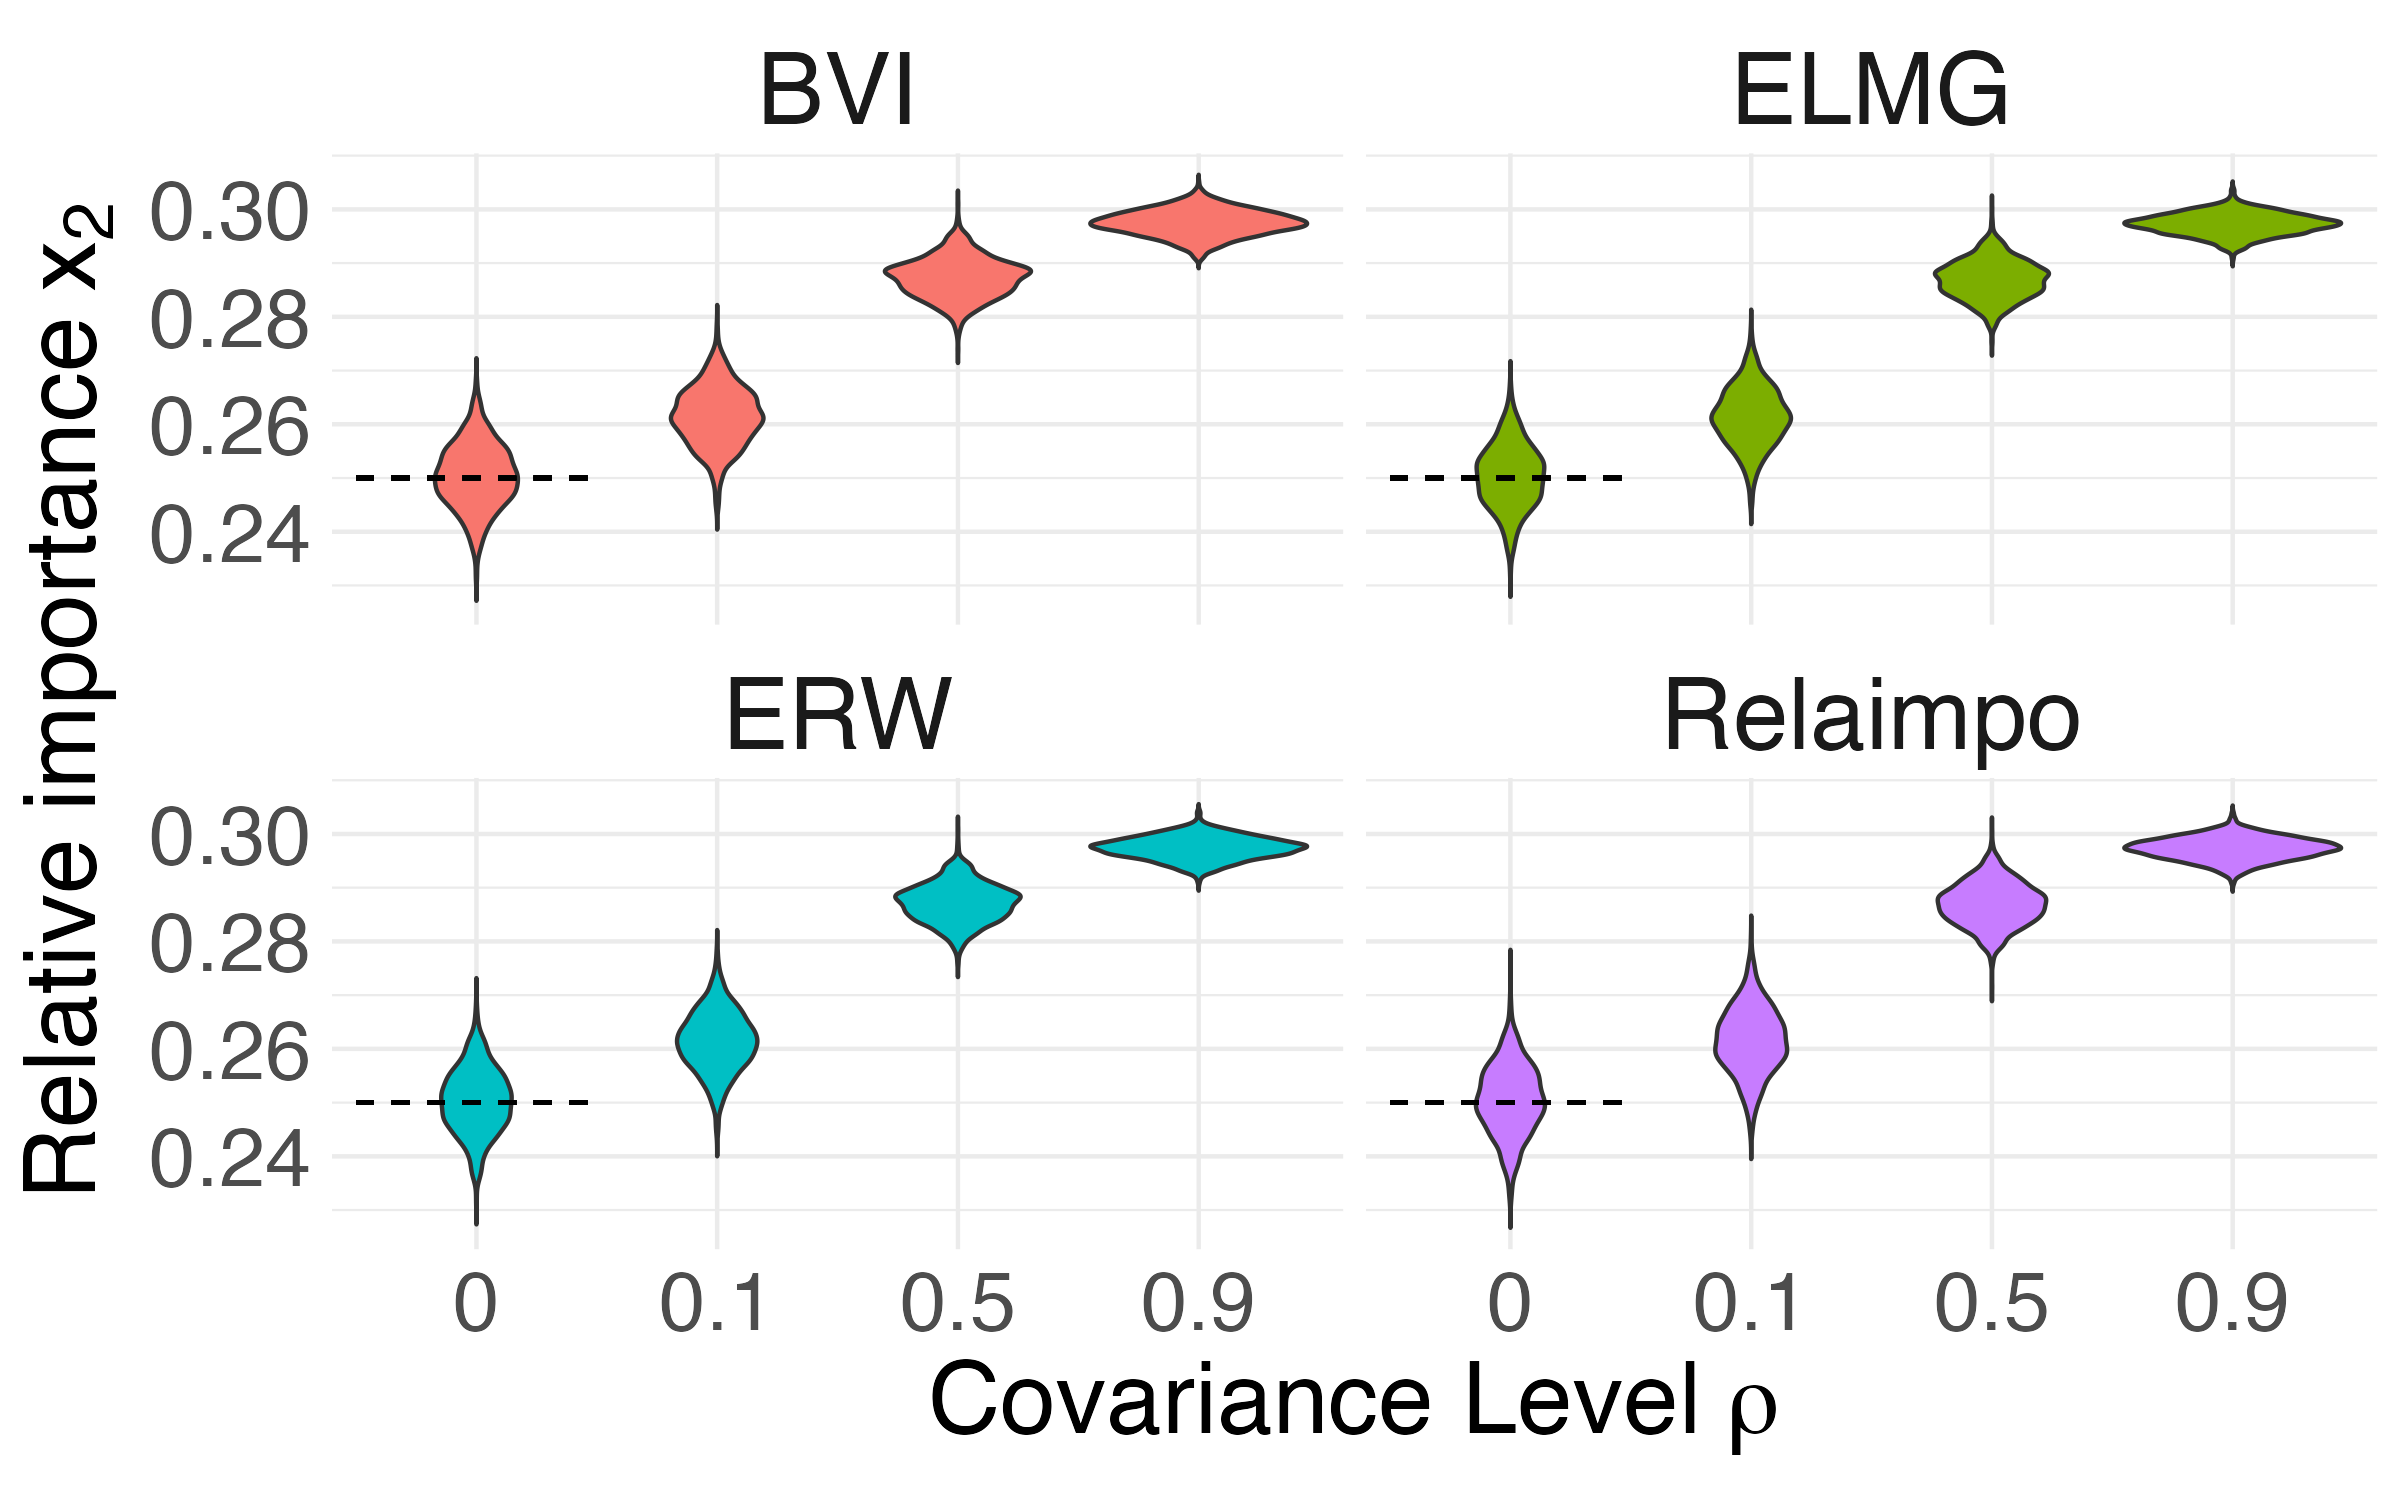
\includegraphics[width=0.6\linewidth]{Figures/ViolinPlots/Variance_V2.png}
%     \label{fig:relimp_X2}
%   }
%   \hfill
%   \subfloat[Relative importance of $X_3$ as calculated from the four methods.]{
%     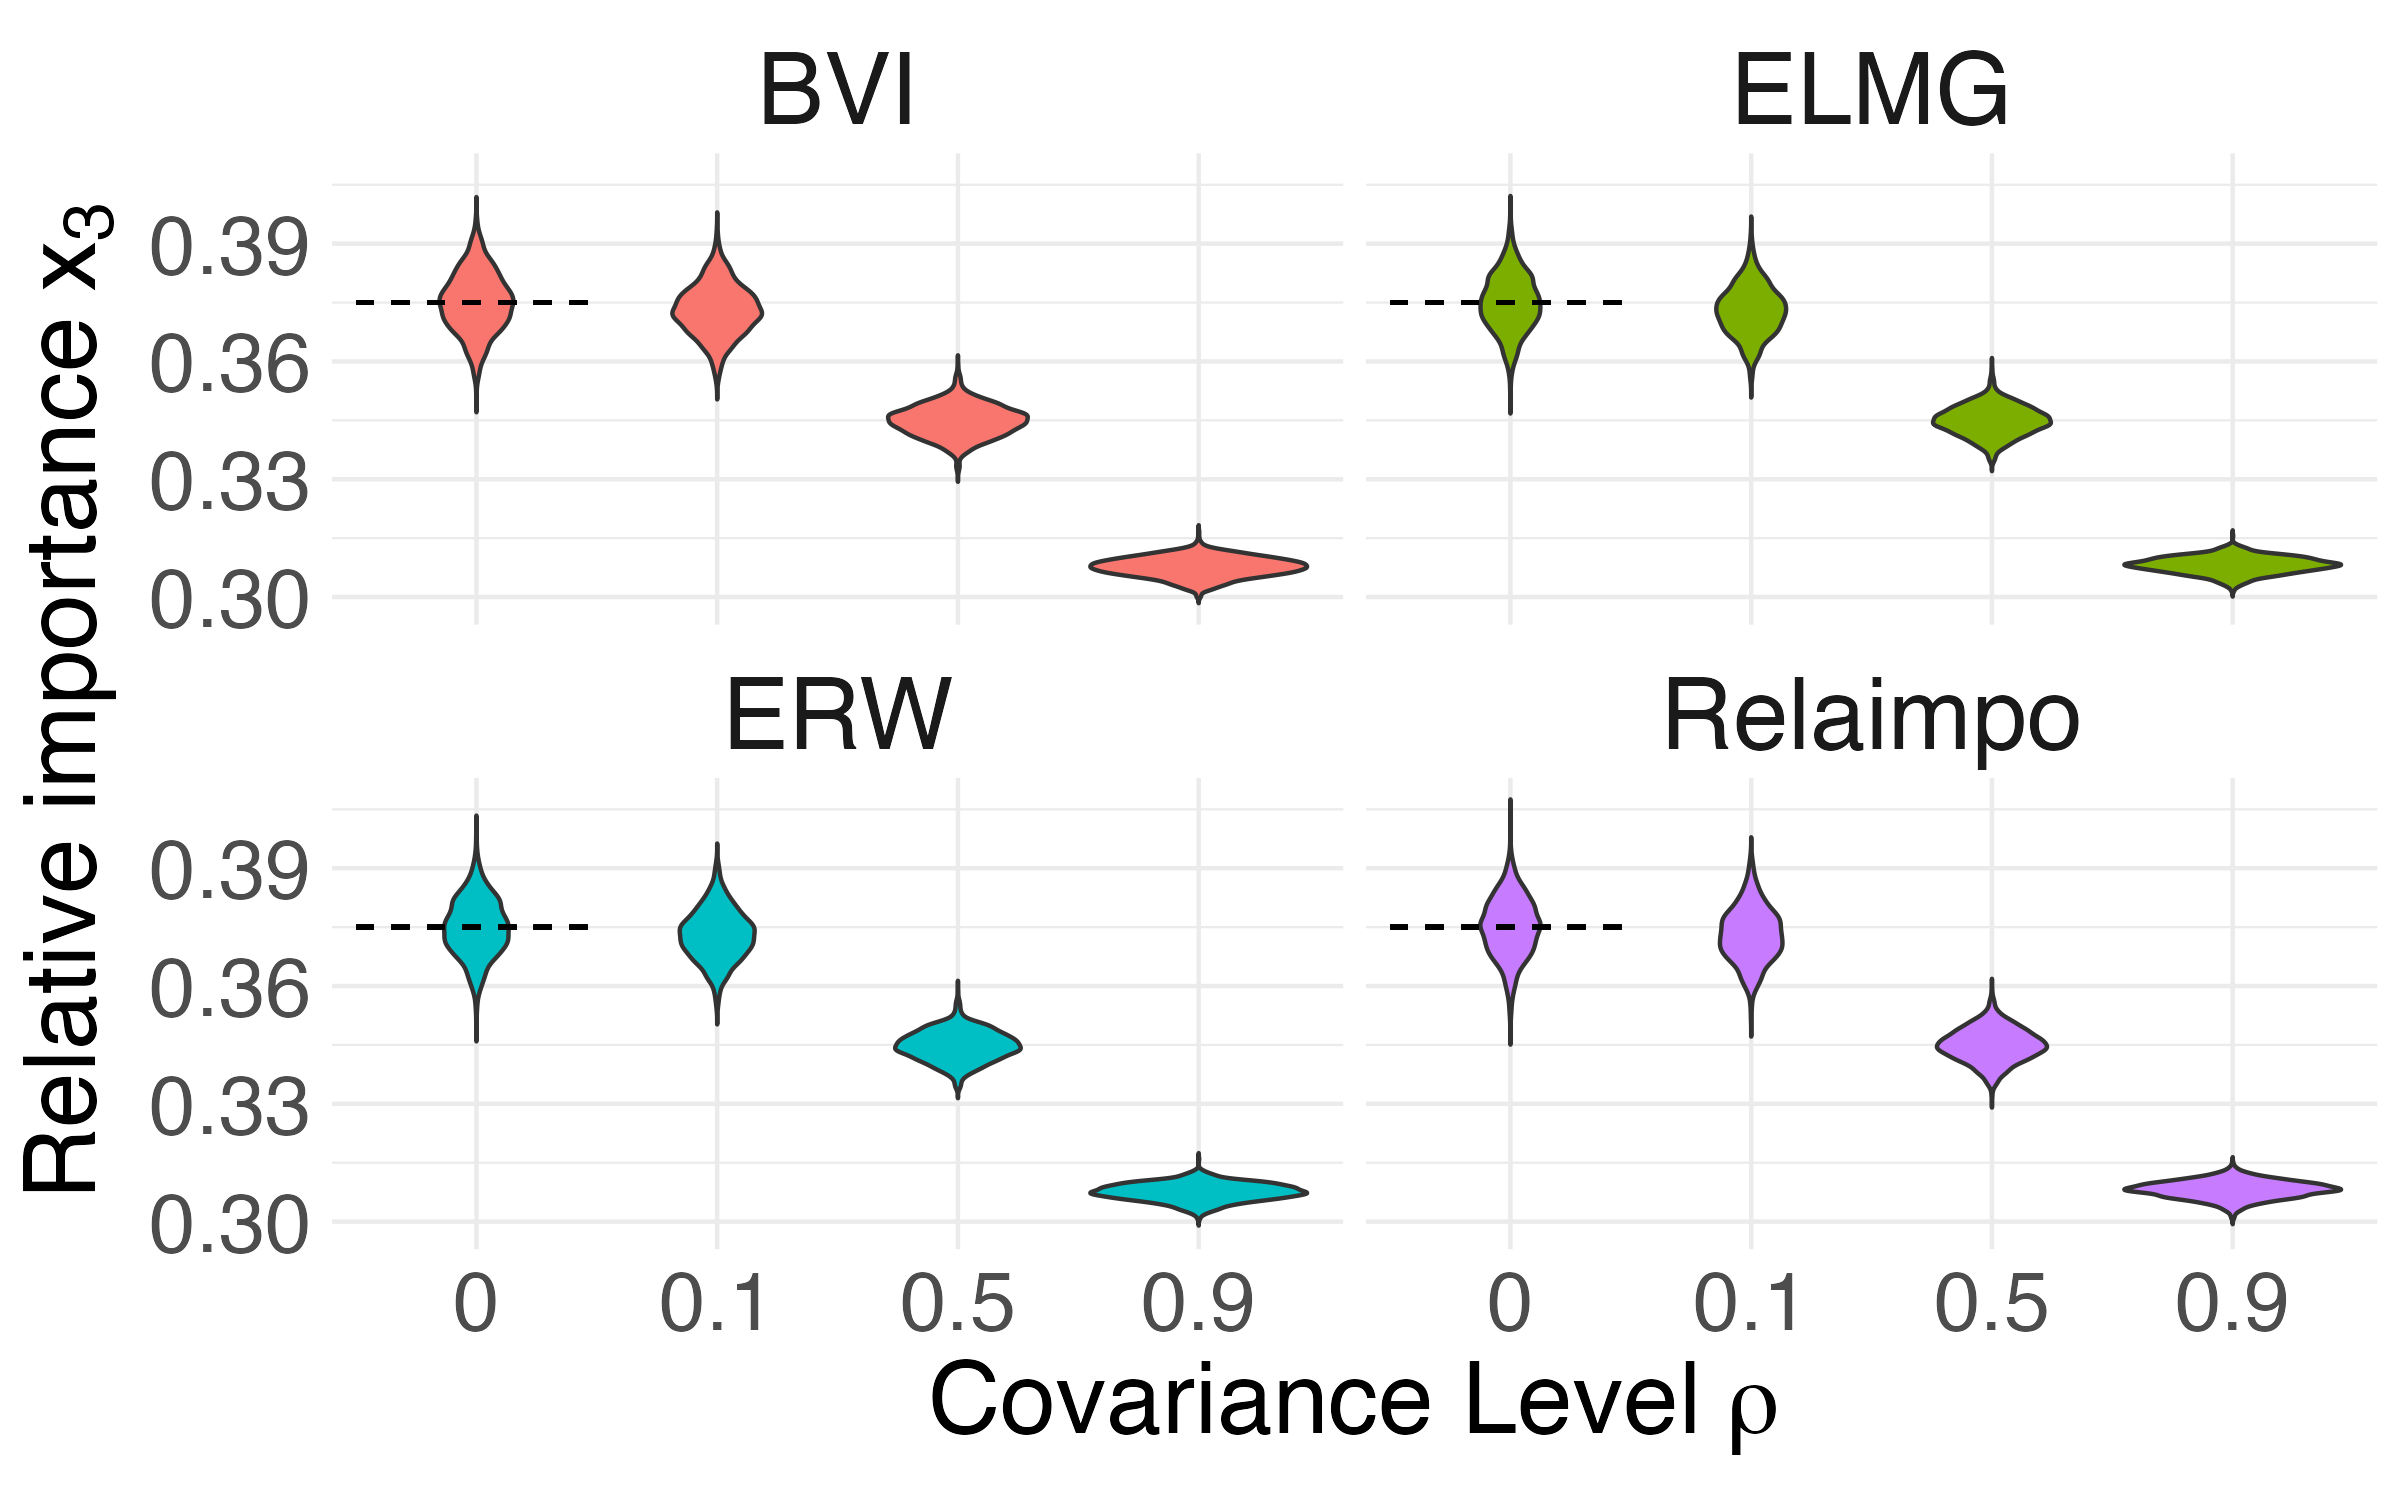
\includegraphics[width=0.6\linewidth]{Figures/ViolinPlots/Variance_V3.png}
%     \label{fig:relimp_X3}
%   }
%   \caption{Violin plots for the relative importance of the fixed effects $X_1, X_2$ and $X_3$ for different correlation levels calculated from $4\cdot 10^4$ simulated datasets by the BVI, ELMG, ERW and the Relaimpo method. The true, standardized regressor coefficients are $\boldsymbol{\beta}=\left(\sqrt{1/8}, \sqrt{2/8}, \sqrt{3/8}\right)$, and the true total model variance is $\sigma^2_{\mathbf{y}}=1$. For the BVI method the posterior means in each simulation are used to compare to the point estimates of the other three methods. The horizontal line displays the theoretically correct importance of each fixed effect in the case of uncorrelated data.}
%   \label{fig:relimp_fixed}
% \end{figure}


% We have, since $\boldsymbol{\Lambda}$ is symmetric, the importances
% \begin{equation} 
%   \begin{aligned}
%     \text{RI}(X_1) &= \boldsymbol{\Lambda}_{1, 1}^{[2]}\beta^{[2]}_1 + \boldsymbol{\Lambda}_{2, 1}^{[2]}\beta^{[2]}_2 + \boldsymbol{\Lambda}_{3, 1}^{[2]}\beta^{[2]}_3 \\ 
%     \text{RI}(X_2) &= \boldsymbol{\Lambda}_{2, 1}^{[2]}\beta^{[2]}_1 + \boldsymbol{\Lambda}_{2, 2}^{[2]}\beta^{[2]}_2 + \boldsymbol{\Lambda}_{3, 2}^{[2]}\beta^{[2]}_3 \\
%     \text{RI}(X_3) &= \boldsymbol{\Lambda}_{3, 1}^{[2]}\beta^{[2]}_1 + \boldsymbol{\Lambda}_{3, 2}^{[2]}\beta^{[2]}_2 + \boldsymbol{\Lambda}_{3, 3}^{[2]}\beta^{[2]}_3 \ ,
%   \end{aligned}
% \end{equation}
% where the columns of $\boldsymbol{\Lambda}^{[2]}$ sum to one. Clearly, if the of diagonal elements increase and the diagonal elements decrease, the importance  


% \begin{table}[!htb]
%   \centering
%   \caption{Your overall caption for all tables.}
%   \label{tab:your-overall-label}
  
%   % First row of tables
%   \begin{minipage}{.45\linewidth}
%   \centering
%   {\footnotesize
%   % latex table generated in R 4.2.1 by xtable 1.8-4 package
% Thu Dec 14 12:52:54 2023
\begin{table}[ht]
\centering
\begin{tabular}{lrrr}
  \hline
Method & Mean & Quantile\_2.5 & Quantile\_97.5 \\ 
  \hline
Relaimpo & 0.284272 & 0.280282 & 0.288313 \\ 
  BVI & 0.284761 & 0.280127 & 0.289150 \\ 
  ELMG & 0.284266 & 0.280411 & 0.288118 \\ 
  ERW & 0.284681 & 0.280541 & 0.288583 \\ 
   \hline
\end{tabular}
\end{table}

%   }
%   \end{minipage}%
%   \hfill
%   \begin{minipage}{.45\linewidth}
%   \centering
%   {\footnotesize
%   % latex table generated in R 4.2.1 by xtable 1.8-4 package
% Thu Dec 14 12:52:54 2023
\begin{table}[ht]
\centering
\begin{tabular}{lrrr}
  \hline
Method & Mean & Quantile\_2.5 & Quantile\_97.5 \\ 
  \hline
Relaimpo & 0.297261 & 0.293124 & 0.301180 \\ 
  BVI & 0.297466 & 0.292623 & 0.302066 \\ 
  ELMG & 0.297251 & 0.293040 & 0.300979 \\ 
  ERW & 0.297389 & 0.293189 & 0.301267 \\ 
   \hline
\end{tabular}
\end{table}

%   }
%   \end{minipage}
  
%   \vspace{5mm} % Adjust the vertical space as needed
  
%   % Second row of tables
%   \begin{minipage}{.45\linewidth}
%   \centering
%   {\footnotesize
%   % latex table generated in R 4.2.1 by xtable 1.8-4 package
% Thu Dec 14 12:52:54 2023
\begin{table}[ht]
\centering
\begin{tabular}{lrrr}
  \hline
Method & Mean & Quantile\_2.5 & Quantile\_97.5 \\ 
  \hline
Relaimpo & 0.308142 & 0.303571 & 0.312266 \\ 
  BVI & 0.307594 & 0.302328 & 0.312071 \\ 
  ELMG & 0.308110 & 0.303704 & 0.312229 \\ 
  ERW & 0.307534 & 0.302991 & 0.311786 \\ 
   \hline
\end{tabular}
\end{table}

%   }
%   \end{minipage}%
%   \hfill
%   \begin{minipage}{.45\linewidth}
%   \centering
%   {\footnotesize
%   % latex table generated in R 4.2.1 by xtable 1.8-4 package
% Thu Dec 14 12:52:54 2023
\begin{table}[ht]
\centering
\begin{tabular}{lrrr}
  \hline
Method & Mean & Quantile\_2.5 & Quantile\_97.5 \\ 
  \hline
Relaimpo &  &  &  \\ 
  BVI & 0.055443 & 0.046108 & 0.066800 \\ 
  ELMG & 0.055070 & 0.045624 & 0.066502 \\ 
  ERW & 0.055094 & 0.044524 & 0.067235 \\ 
   \hline
\end{tabular}
\end{table}

%   }
%   \end{minipage}
  
% \end{table}
  
  
% \end{table}
% % latex table generated in R 4.2.1 by xtable 1.8-4 package
% Thu Dec 14 12:52:54 2023
\begin{table}[ht]
\centering
\begin{tabular}{lrrr}
  \hline
Method & Mean & Quantile\_2.5 & Quantile\_97.5 \\ 
  \hline
Relaimpo & 0.284272 & 0.280282 & 0.288313 \\ 
  BVI & 0.284761 & 0.280127 & 0.289150 \\ 
  ELMG & 0.284266 & 0.280411 & 0.288118 \\ 
  ERW & 0.284681 & 0.280541 & 0.288583 \\ 
   \hline
\end{tabular}
\end{table}

% % latex table generated in R 4.2.1 by xtable 1.8-4 package
% Thu Dec 14 12:52:54 2023
\begin{table}[ht]
\centering
\begin{tabular}{lrrr}
  \hline
Method & Mean & Quantile\_2.5 & Quantile\_97.5 \\ 
  \hline
Relaimpo & 0.297261 & 0.293124 & 0.301180 \\ 
  BVI & 0.297466 & 0.292623 & 0.302066 \\ 
  ELMG & 0.297251 & 0.293040 & 0.300979 \\ 
  ERW & 0.297389 & 0.293189 & 0.301267 \\ 
   \hline
\end{tabular}
\end{table}

% % latex table generated in R 4.2.1 by xtable 1.8-4 package
% Thu Dec 14 12:52:54 2023
\begin{table}[ht]
\centering
\begin{tabular}{lrrr}
  \hline
Method & Mean & Quantile\_2.5 & Quantile\_97.5 \\ 
  \hline
Relaimpo & 0.308142 & 0.303571 & 0.312266 \\ 
  BVI & 0.307594 & 0.302328 & 0.312071 \\ 
  ELMG & 0.308110 & 0.303704 & 0.312229 \\ 
  ERW & 0.307534 & 0.302991 & 0.311786 \\ 
   \hline
\end{tabular}
\end{table}

% Displayed in figure \ref{fig:relimp_fixed} are the calculated relative importances for the fixed effects for different covariance levels, along with the theoretically correct value when the data are uncorrelated as a dashed line. 
% %Rewrite the above sentence

% %Go thorugh each plot for the different regressors as below and discuss and compare all methods.
% For $X_1$ the relative importance is $\beta_1^2$ and we see in \ref{fig:relimp_X1} that all methods are consistent when the data are uncorrelated, giving a violin that is evenly distributed about the correct value $\frac{1}{8} = 0.125$.

%In general, our method produces results that are very similar to that of established methods for the fixed effects, and follows the same trends. 
%Should I make the limits of the plots tighter so that the violins become bigger? The problem then is that we lose the same axis.

\subsection{Relative importance of the random effects}
\label{sec:relimp_random}
Considering a model with one random intercept, we can no longer compare our model with the Relaimpo method, which is only implemented for the linear regression in the relaimpo R package \citep{gromping_relaimpo}. Therefore, we now compare the BVI method only with the ELMG and ERW methods, which have been extended from the Relaimpo method \citep{matre}.
\Cref{fig:relimp_alpha} shows the distribution of the relative importance, or variance, assigned to the random intercept $\boldsymbol{\alpha}$ for different correlation levels. 
The random intercept $\boldsymbol{\alpha}$ follows a univariate normal distribution with variance equal to $1/8$ and the standard deviation of the response is $\sigma^2_{\mathbf{y}}=1$. 
As before the horizontal line shows the theoretical relative importance that $\boldsymbol{\alpha}$ has in the model when the fixed effects are uncorrelated.
\newline
\newline
From \Cref{fig:relimp_alpha} it is apparent that both the location and width of the relative importance distribution of all methods are largely indistinguishable. 
The distributions take on a moderately smaller value when $\rho=0.1$ and the location of the estimates is further decreased for $\rho=0.5$ and $\rho=0.9$. 
For the latter correlation level, the distributions are located around a value that is less than half of the value of the centering when the fixed effects are uncorrelated. 
To re-emphasize, this is both expected and desirable since the increase in response variance comes solely from the correlation of fixed effects, so the random effects now contribute to explain a smaller proportion of the variance, \textit{i.e.} the importance is lower.
\begin{figure}[ht]
  \centering
  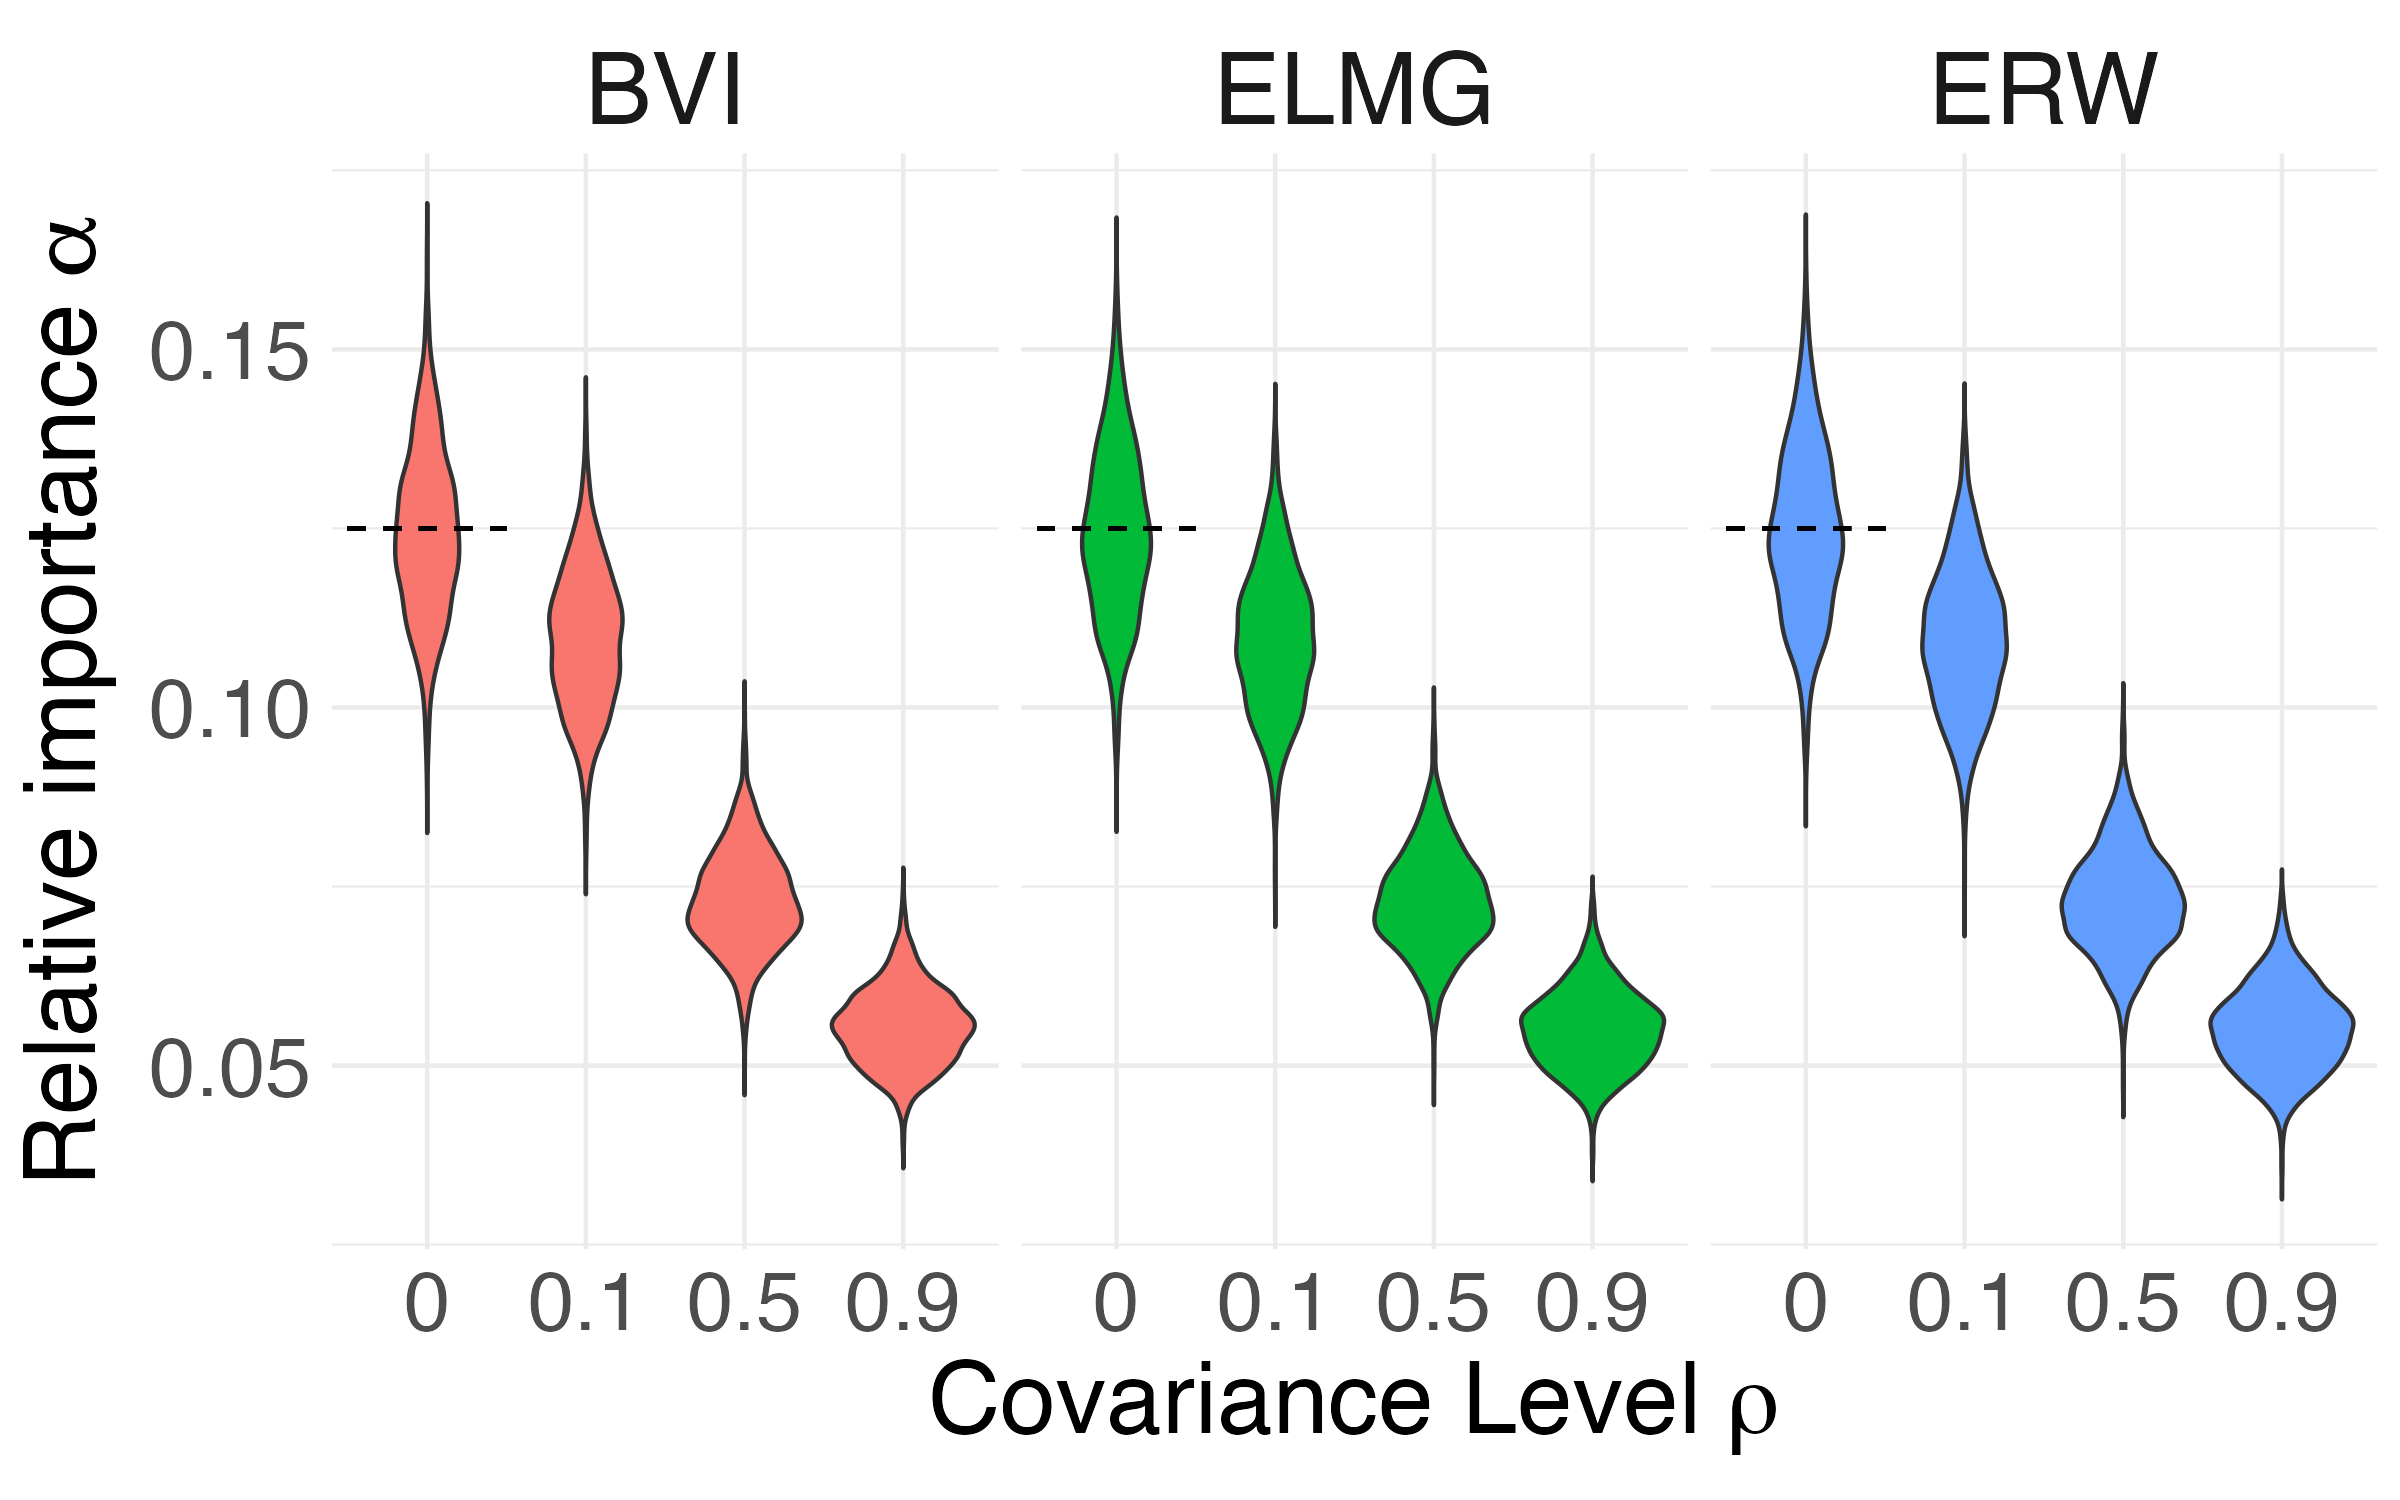
\includegraphics[width=0.7\linewidth]{Figures/ViolinPlots/Variance_gamma.png}
  \caption{Violin plots for the relative importance of the random effect $\boldsymbol{\alpha}$, that is, $\hat{\sigma}^2_{\alpha}$ for different correlation levels calculated from the ensemble of simulated datasets by the BVI, ELMG and the ERW method. For the BVI method the distributions of posterior means of the marginal distribution of $\hat{\sigma}^2_{\alpha}$ are shown to compare to the point estimates of the other two methods. The horizontal line displays the theoretically correct importance $\sigma^2_{\alpha} = 0.125$ of the random effect in the case of uncorrelated data.}
  \label{fig:relimp_alpha}
\end{figure}

\subsection{Total variance explained - $R^2$ estimates}
\label{sec:R2} 
As a useful by-product from the previous results we can get the total variances explained by our model (\Cref{fig:total_variance}).
The marginal variance explained is the variance explained by the fixed effects (\Cref{fig:variance_marginal}), and we get results for all four methods, including Relaimpo.
In \Cref{fig:variance_conditional} the total conditional variance explained, $R^2_{\text{cond}}$, is displayed. 
This is the variance given all the fixed effects and the random effect.
To complement the conditional and marginal variances explained, a horizontal line is drawn for each correlation level corresponding to the theoretically correct variance explained, found in \Cref{table:1}, for the correlation level. 
\newline
\newline
\Cref{fig:variance_marginal} shows that the four methods produce very similar results of $R^2_{\text{marg}}$ for the fixed effects across all correlation values, albeit a slightly larger width for the BVI method can be seen.
When considering the conditional variance $R^2_{\text{cond}}$ in \Cref{fig:variance_conditional}, the dispersion of the BVI method is strikingly larger compared to the other methods. 
It is not immediately clear why, but it could be due to the dispersion of the estimated posterior marginal variance of $\boldsymbol{\alpha}$ which will be presented in \Cref{sec:posterior_distributions}.
Both the marginal and the conditional variance are centered around the theoretically correct value with some variability, particularly visible for conditional variance of the BVI method. 
The centering of the distributions for both the marginal and conditional variances resemble each other for all methods, regardless of correlation level.
\begin{figure}[!ht]
  \centering
  % First row
  \subfloat[Total marginal variance $R^2_{\text{marg}}$.]{
    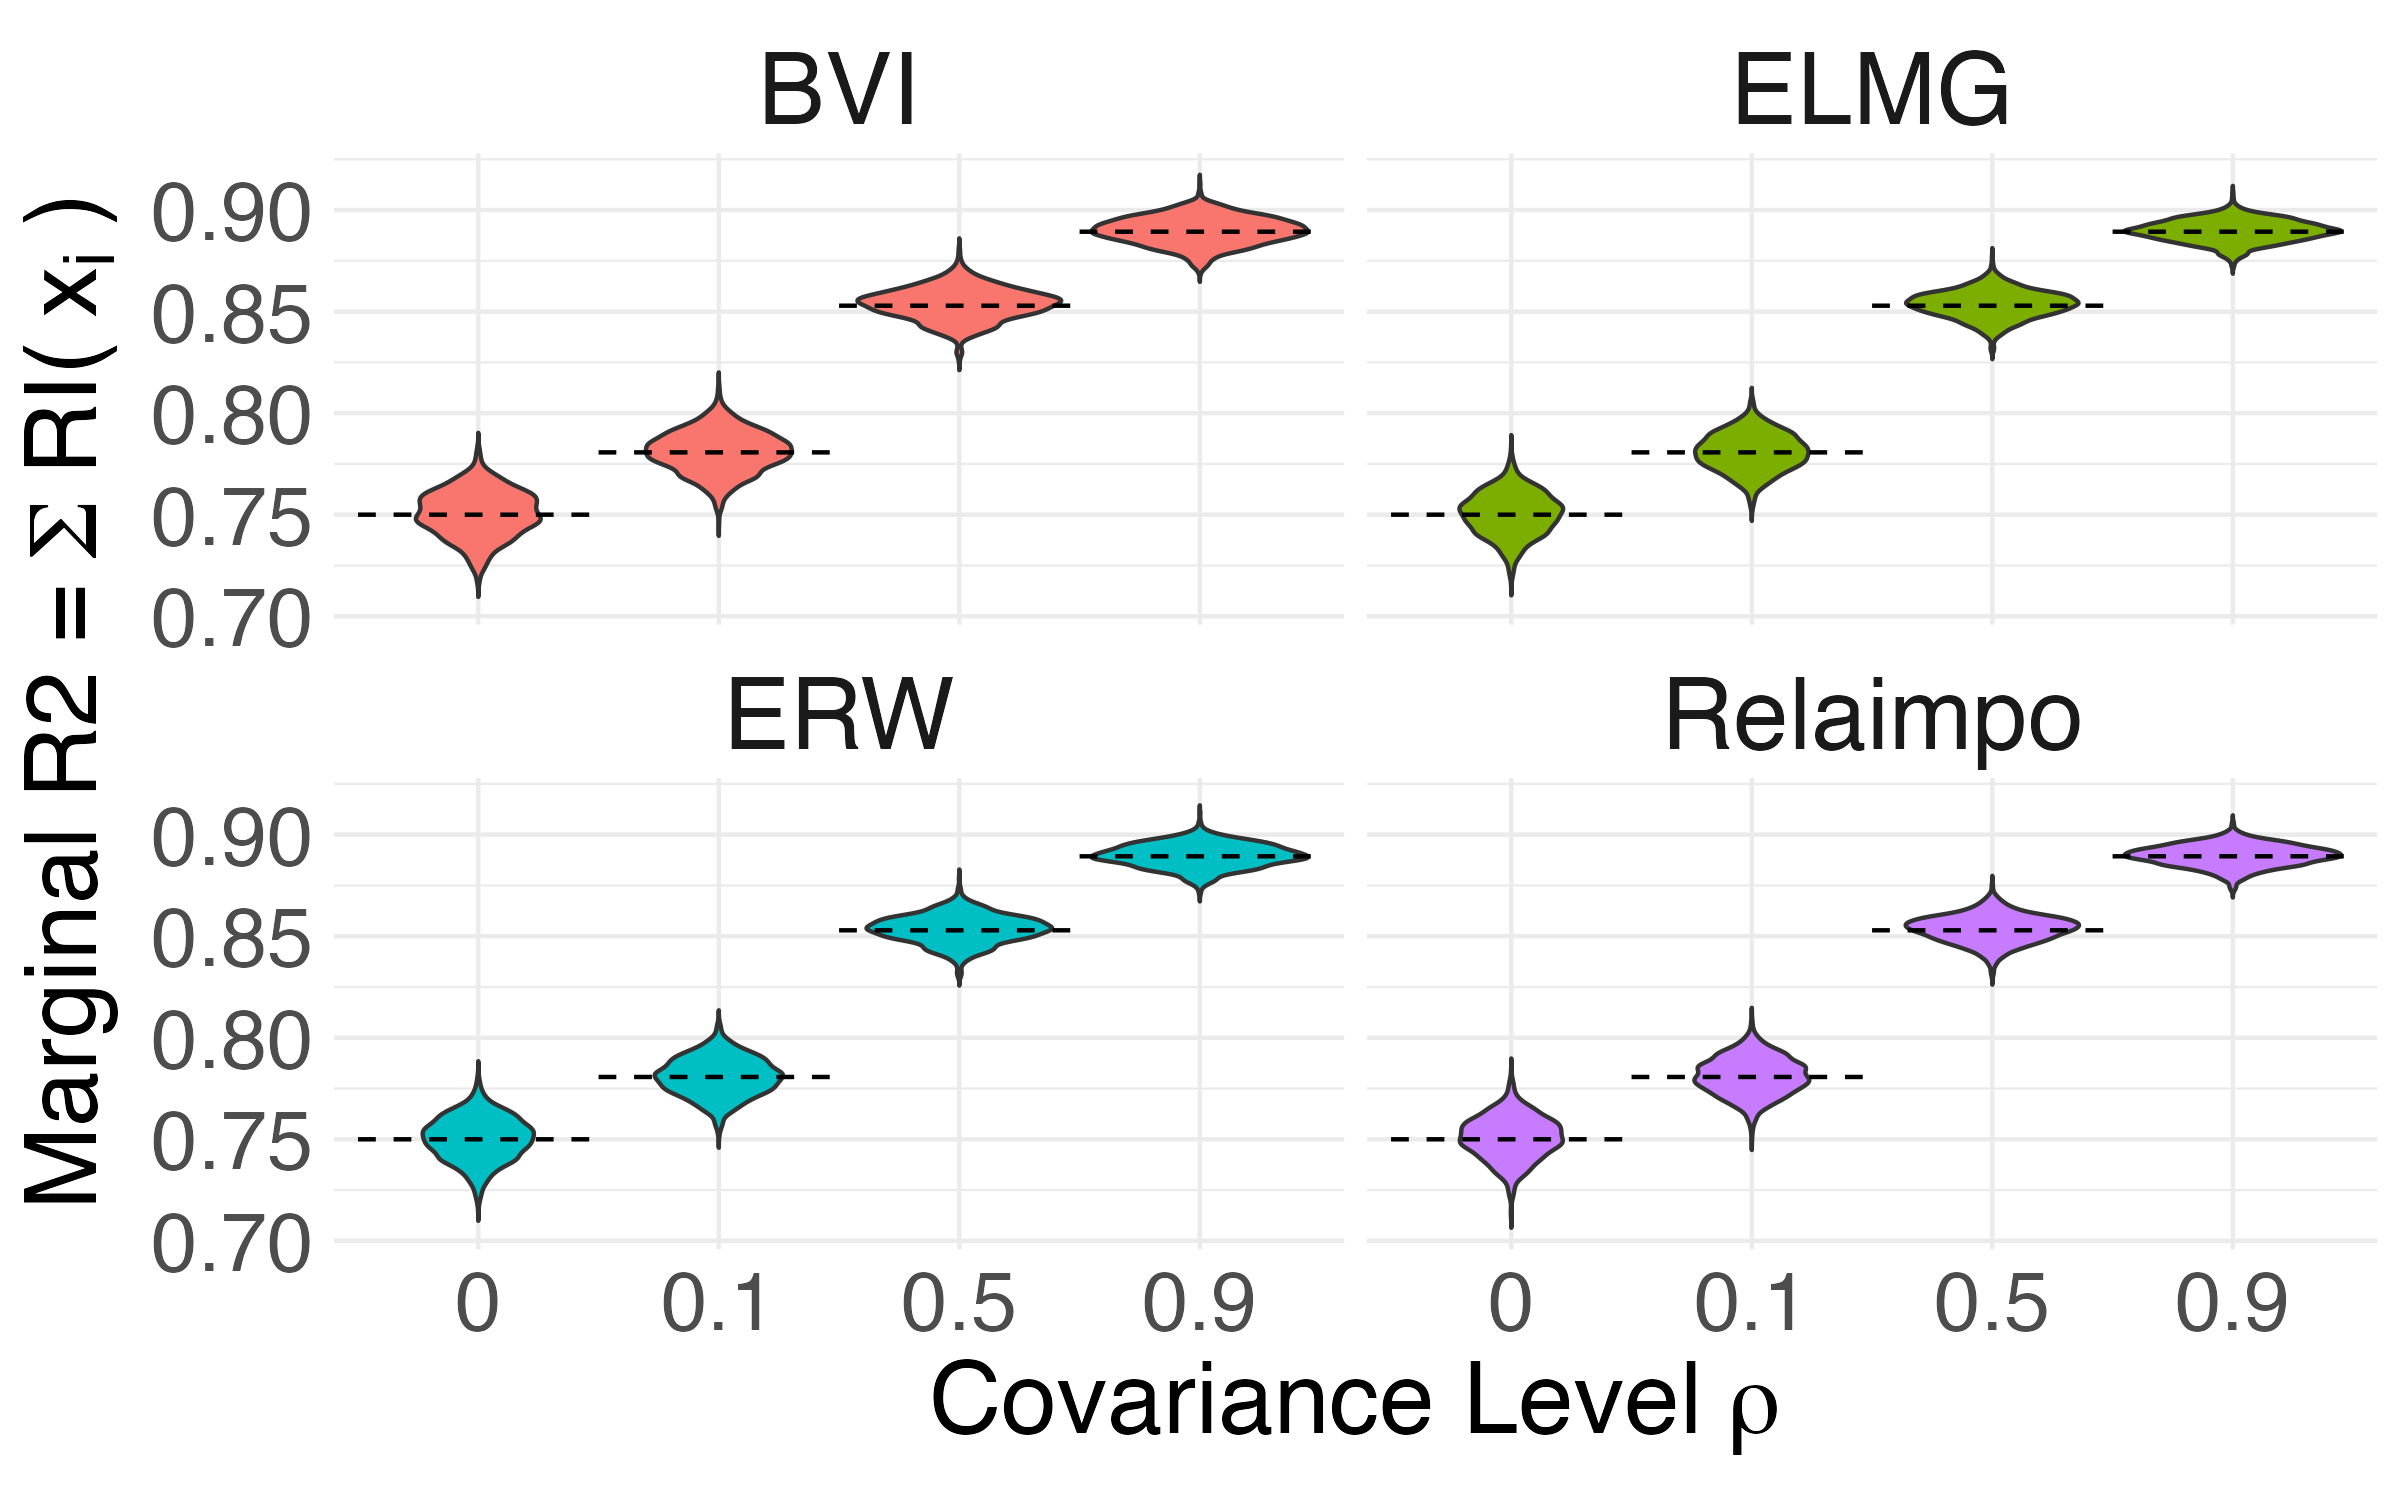
\includegraphics[width=0.6\linewidth]{Figures/ViolinPlots/Marginal_Variance.png}
    \label{fig:variance_marginal}
  }
  \hfill
  \subfloat[Total conditional variance $R^2_{\text{cond}}$.]{
    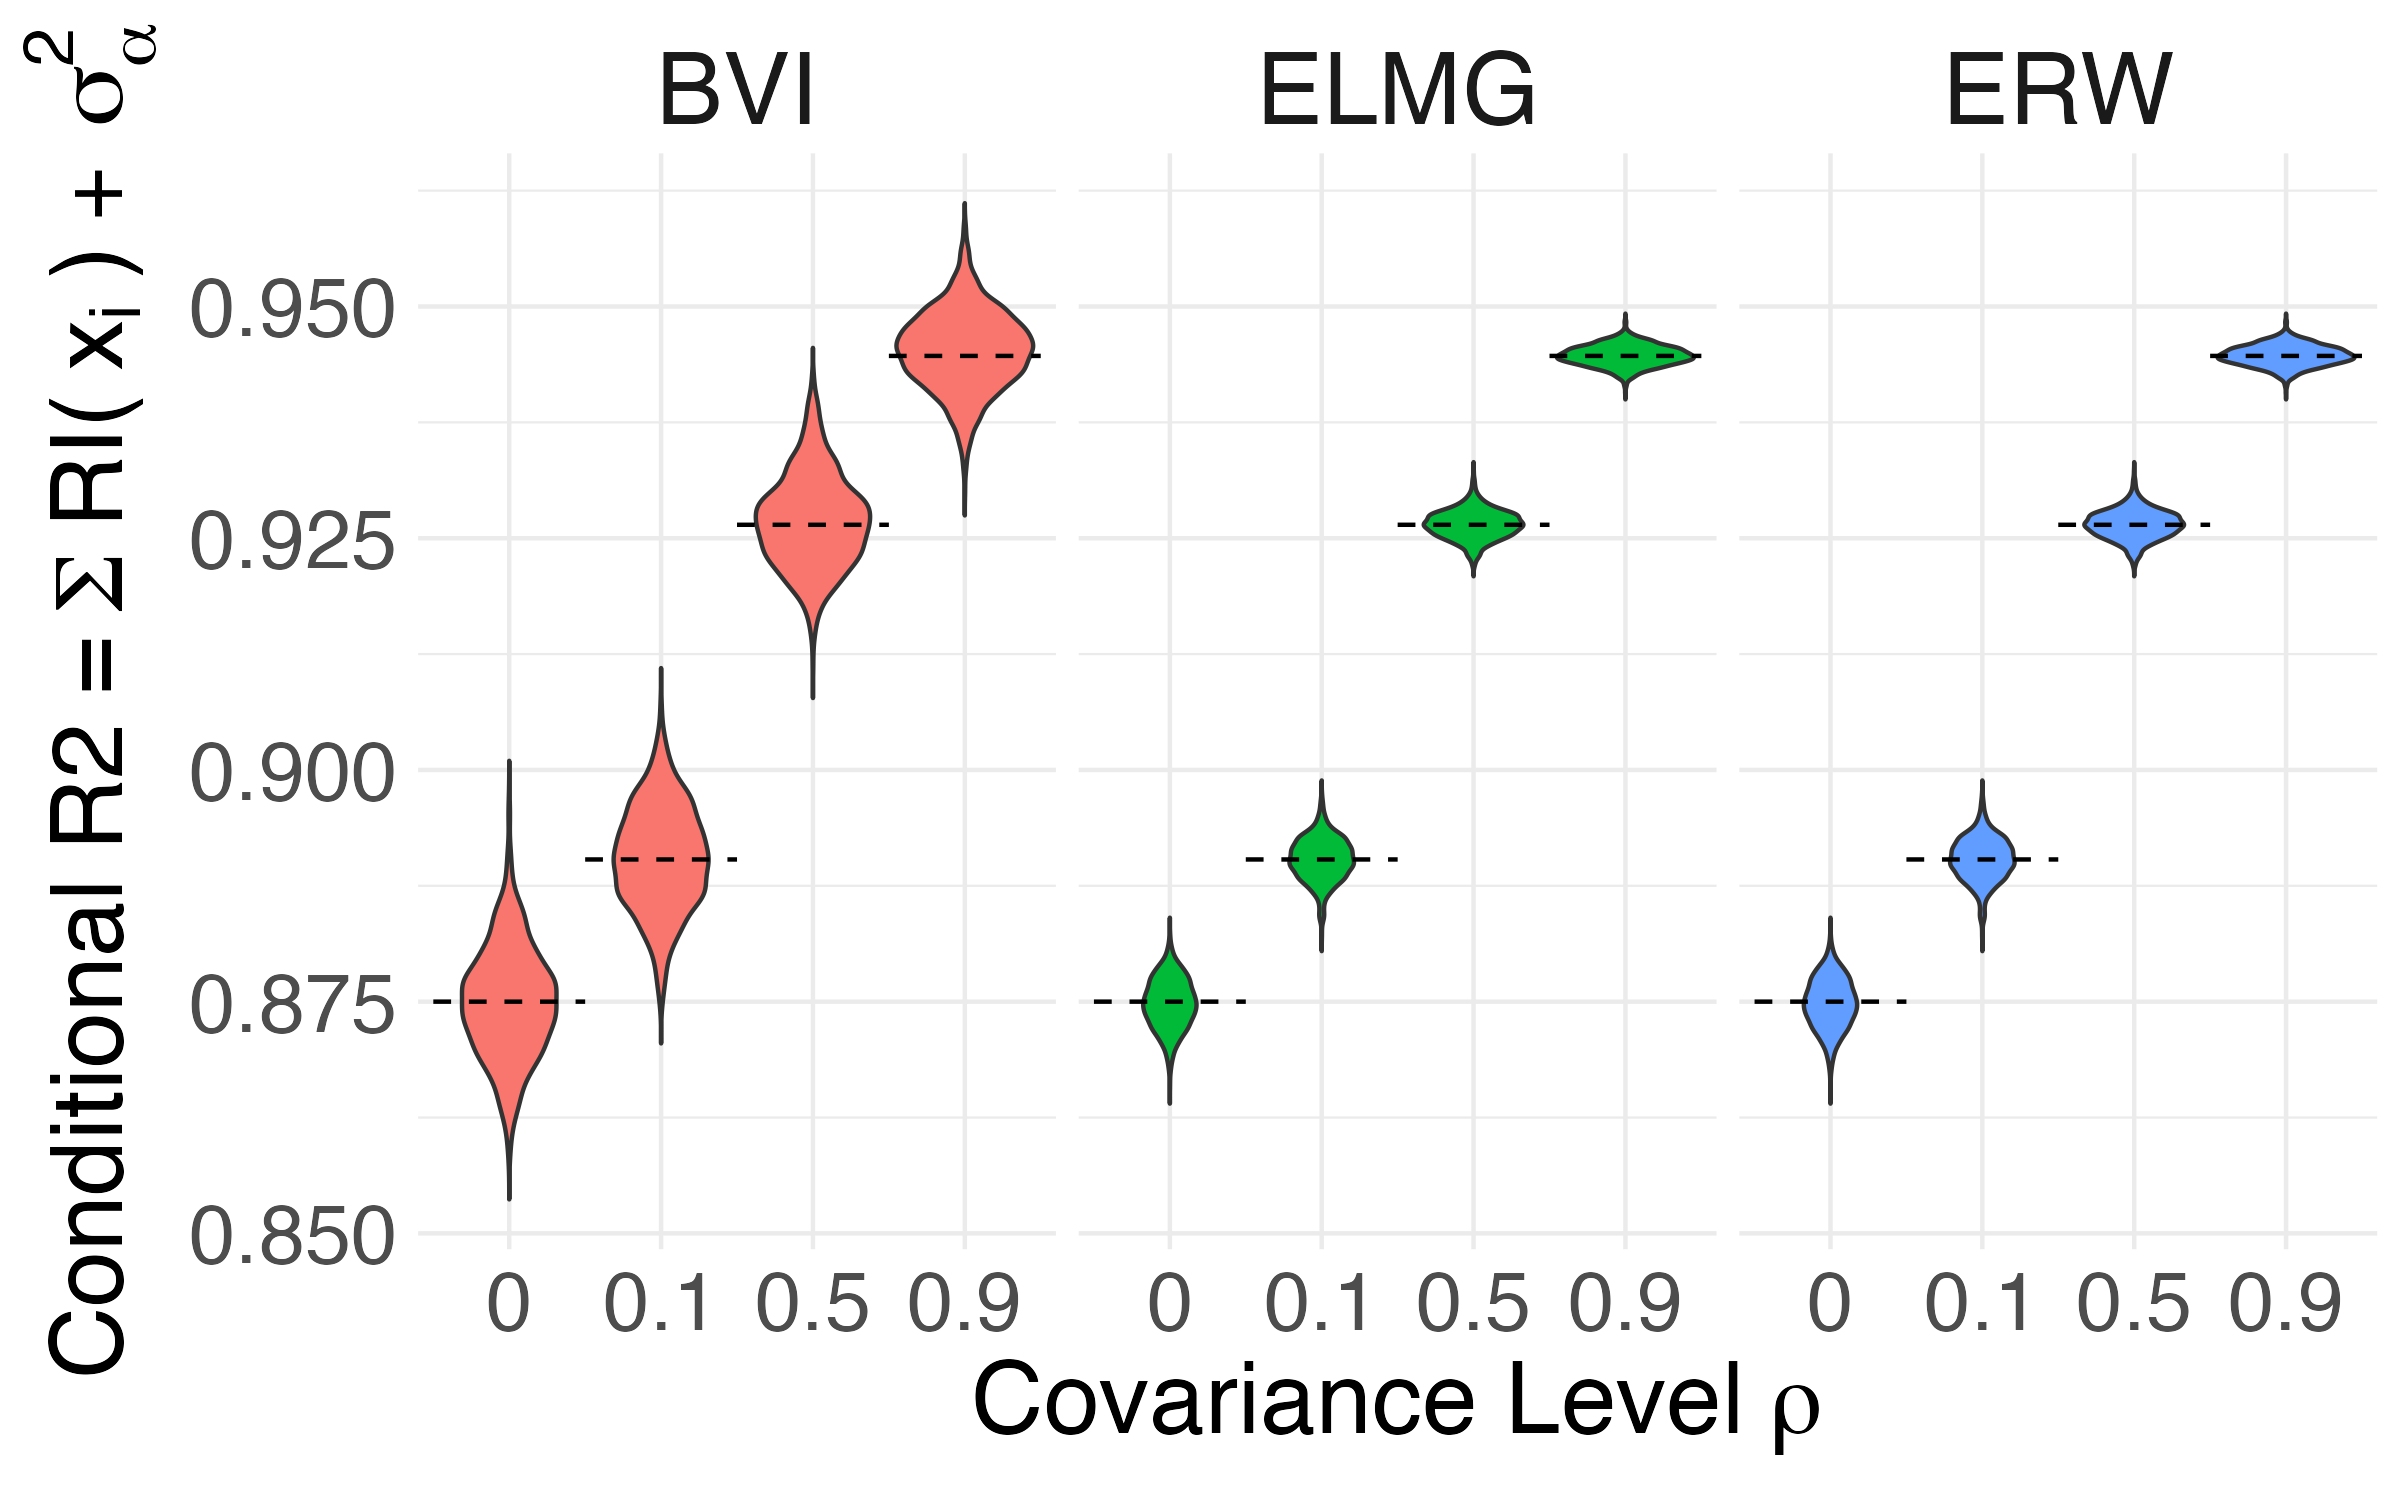
\includegraphics[width=0.6\linewidth]{Figures/ViolinPlots/Conditional_Variance.png}
    \label{fig:variance_conditional}
  }
  \caption{Violin plots for the total marginal and conditional variance explained for different correlation levels calculated from the ensemble of simulated datasets by the BVI, ELMG, the ERW and the Relaimpo method(only marginal variance explained can be computed). For the BVI method the posterior means of the sampled posterior distributions of $\boldsymbol{\beta}$ and the marginal distribution of $\hat{\sigma}^2_{\alpha}$ in each simulation are used to compare to the point estimates of the other two methods. The horizontal lines display the theoretical explained variance for each correlation level $\rho$ as in \Cref{table:1}.}
  \label{fig:total_variance}
\end{figure}

\newpage
\section{The BVI method}
The results from the BVI method for each dataset consists of the posterior marginal distributions of the variances of $\boldsymbol{\alpha}$ and $\boldsymbol{\varepsilon}$, as well as the approximated distribution of $\text{RI}(\mathbf{X})$ from samples $\boldsymbol{\beta}_{s, \mathbf{Z}}$ drawn from the joint posterior distribution $\pi(\boldsymbol{\beta}_{\mathbf{Z}}, \boldsymbol{\alpha} \lvert \mathbf{y})$.
The derivation of these results are described in detail in \Cref{sec:BVI_handling} and provides a more informative basis to make inference on compared to point estimation.
As this is the key advantage of the Bayesian framework, we also take a look on what results our method provides for a single model fit for different correlation levels. 
We calculate these posterior distributions for the same four different correlation levels as we use in the simulation study.
Further, we use the samples $\boldsymbol{\beta}_{s, \mathbf{Z}}$ from the joint distribution and the marginal posterior variances of $\boldsymbol{\alpha}$ and $\boldsymbol{\varepsilon}$ to calculate the distribution of $R^2$ in accordance with \eqref{eq:R2_bayes_LMM_cond} and \eqref{eq:R2_bayes_LMM_marg}. 

\subsection{Posterior relative importance distributions}
\label{sec:posterior_distributions}
Approximate posterior marginal distributions for the variances of the random effects, and sampled approximate posterior distributions for the fixed effects are available for the BVI method for each dataset.
These are featured in \Cref{fig:posterior_distributions} for one realization of the four different datasets of different correlations.
All posteriors for one correlation level are shown in the same subplot, with one subplot for each correlation level. 
For the correlation level $\rho=0$ the theoretically correct relative importances are shown as vertical lines.
Note here that it is expected and desired that the distributions from a single dataset are stochastic and therefore deviate somewhat from the theoretical values.
When data are uncorrelated (\Cref{fig:posteriors_none}) the posterior distributions are coincidentally centered close to the theoretical value.
The posterior distribution of $\hat{\sigma}^2_{\alpha}$ is slightly skewed to the left and demonstrates a distinctively larger degree of dispersion than the other effects.
For $\rho=0.1$ (\Cref{fig:posteriors_low}), a small shift of all posterior distributions is noticeable, in accordance with the results from \Cref{fig:relimp_X1} and \Cref{fig:relimp_alpha}. 
This repositioning is more clear for $\rho=0.5$ and $\rho=0.9$ (\Cref{fig:posteriors_medium} and \Cref{fig:posteriors_high}), and it is clear to see that the posterior distribution of the variance of $\hat{\sigma}^2_{\alpha}$ follows the trend of $\hat{\sigma}^2_{\varepsilon}$ closely.
When correlation is increased, it seems that the width of all posterior distributions narrow and become tighter.
The trend of increasing relative importance assigned to $X_1$ and $X_2$ while decreasing importance assigned to $X_3$ is highlighted by the posterior distributions of the respective effects as they align closer for each increase in correlation.
These are the types of results that we would expect to see, as they deviate from the theoretical values with a plausible amount when considering that they are stochastic.
\begin{figure}[!ht]
  \centering
  % First row
  \subfloat[$\rho=0$]{
    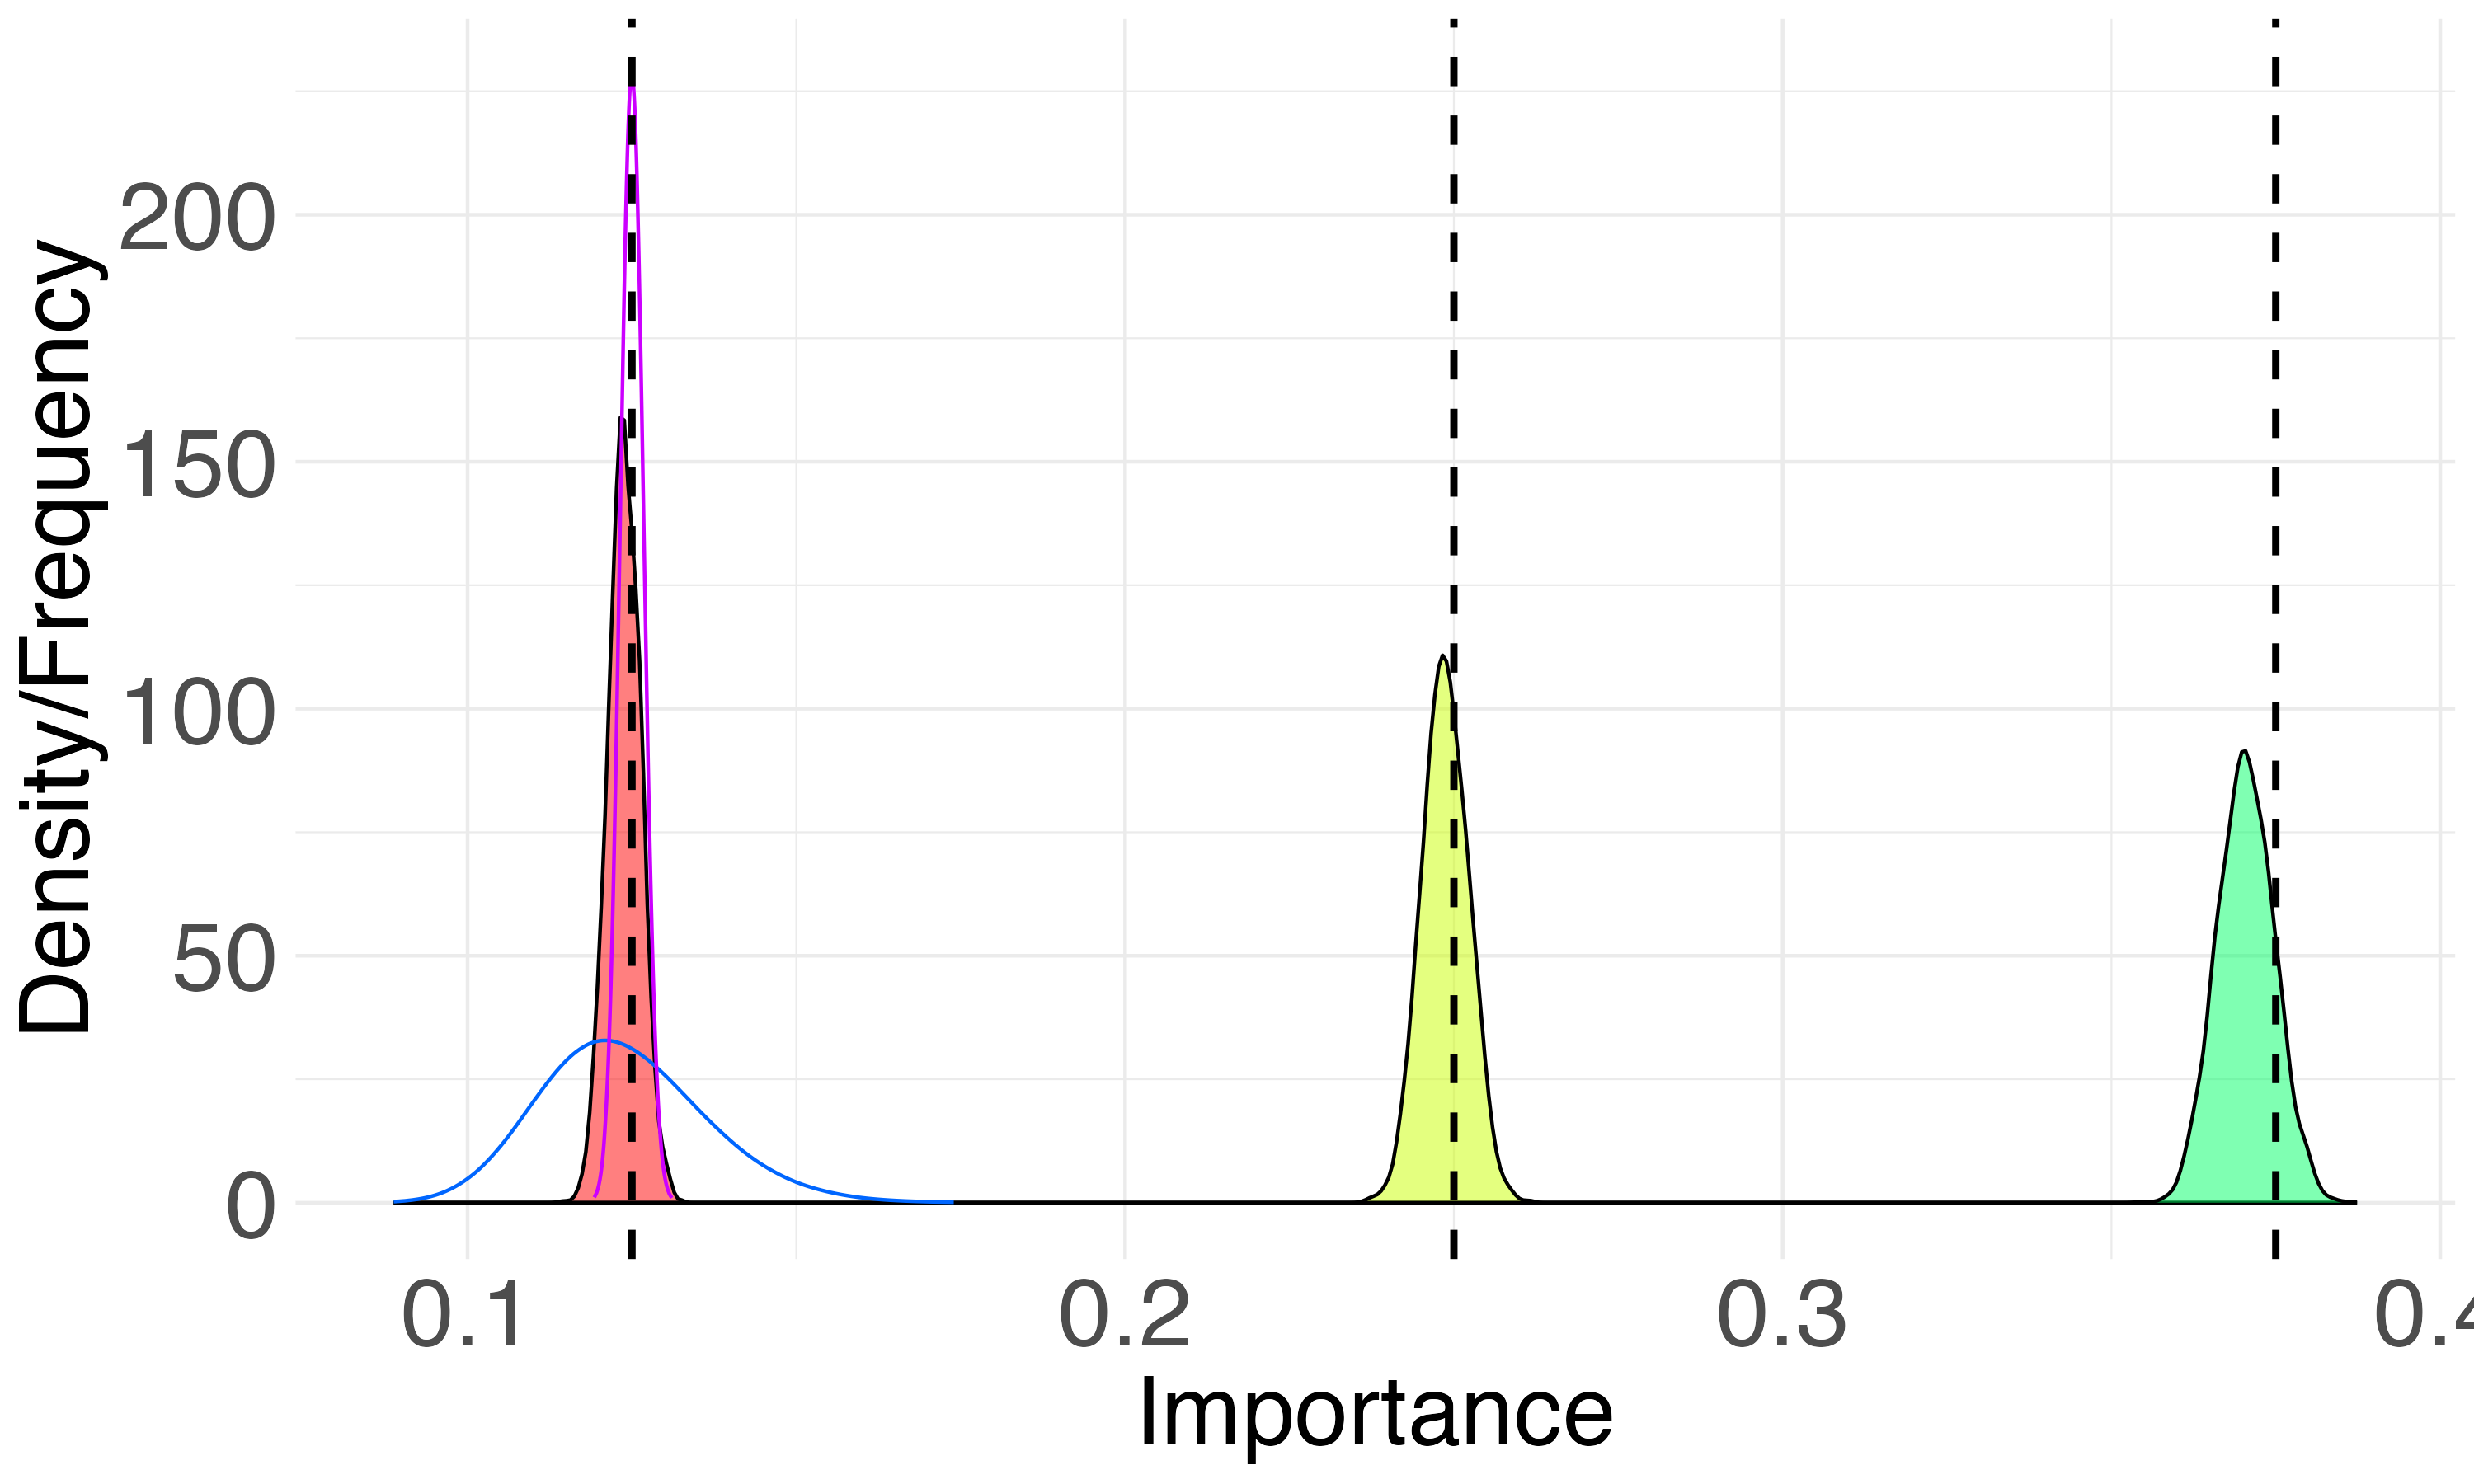
\includegraphics[width=0.5\linewidth]{Figures/Posterior Marginal/Posterior importance, cov=none.png}
    \label{fig:posteriors_none}
  }
  \subfloat[$\rho=0.1$]{
    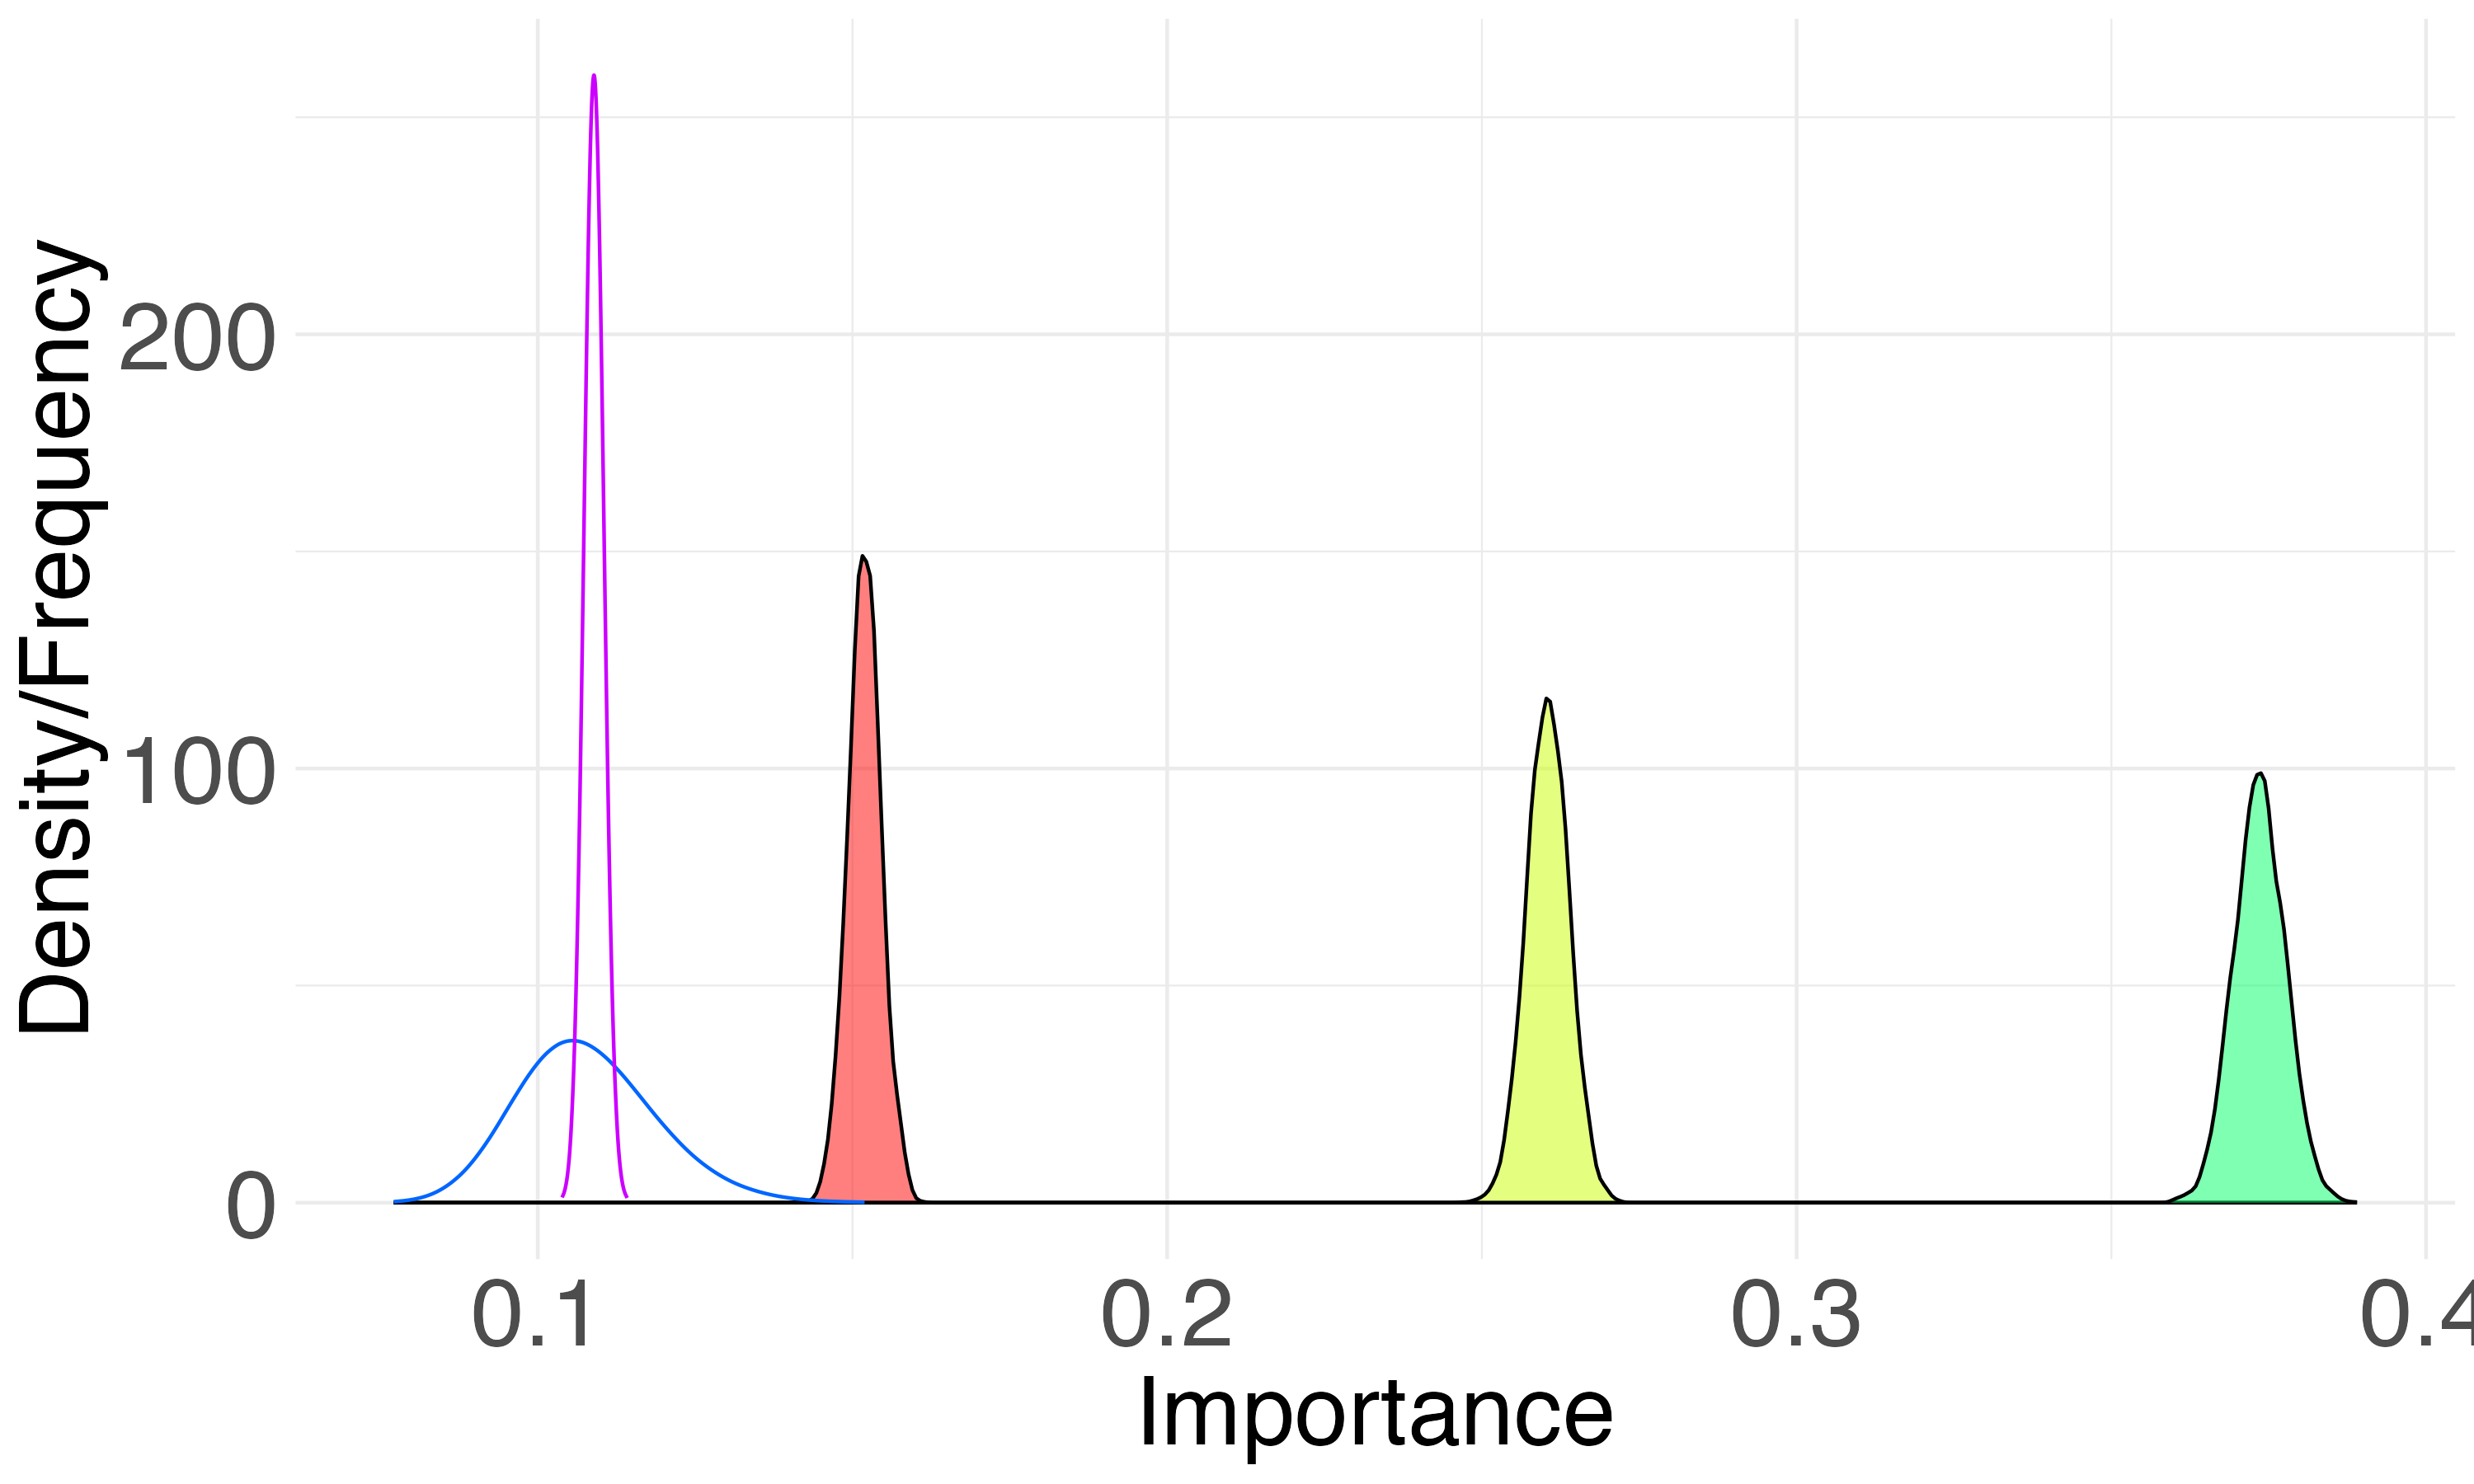
\includegraphics[width=0.5\linewidth]{Figures/Posterior Marginal/Posterior importance, cov=low.png}
    \label{fig:posteriors_low}
  }
  \vspace{5mm}
  % Second row
  \subfloat[$\rho=0.5$]{
    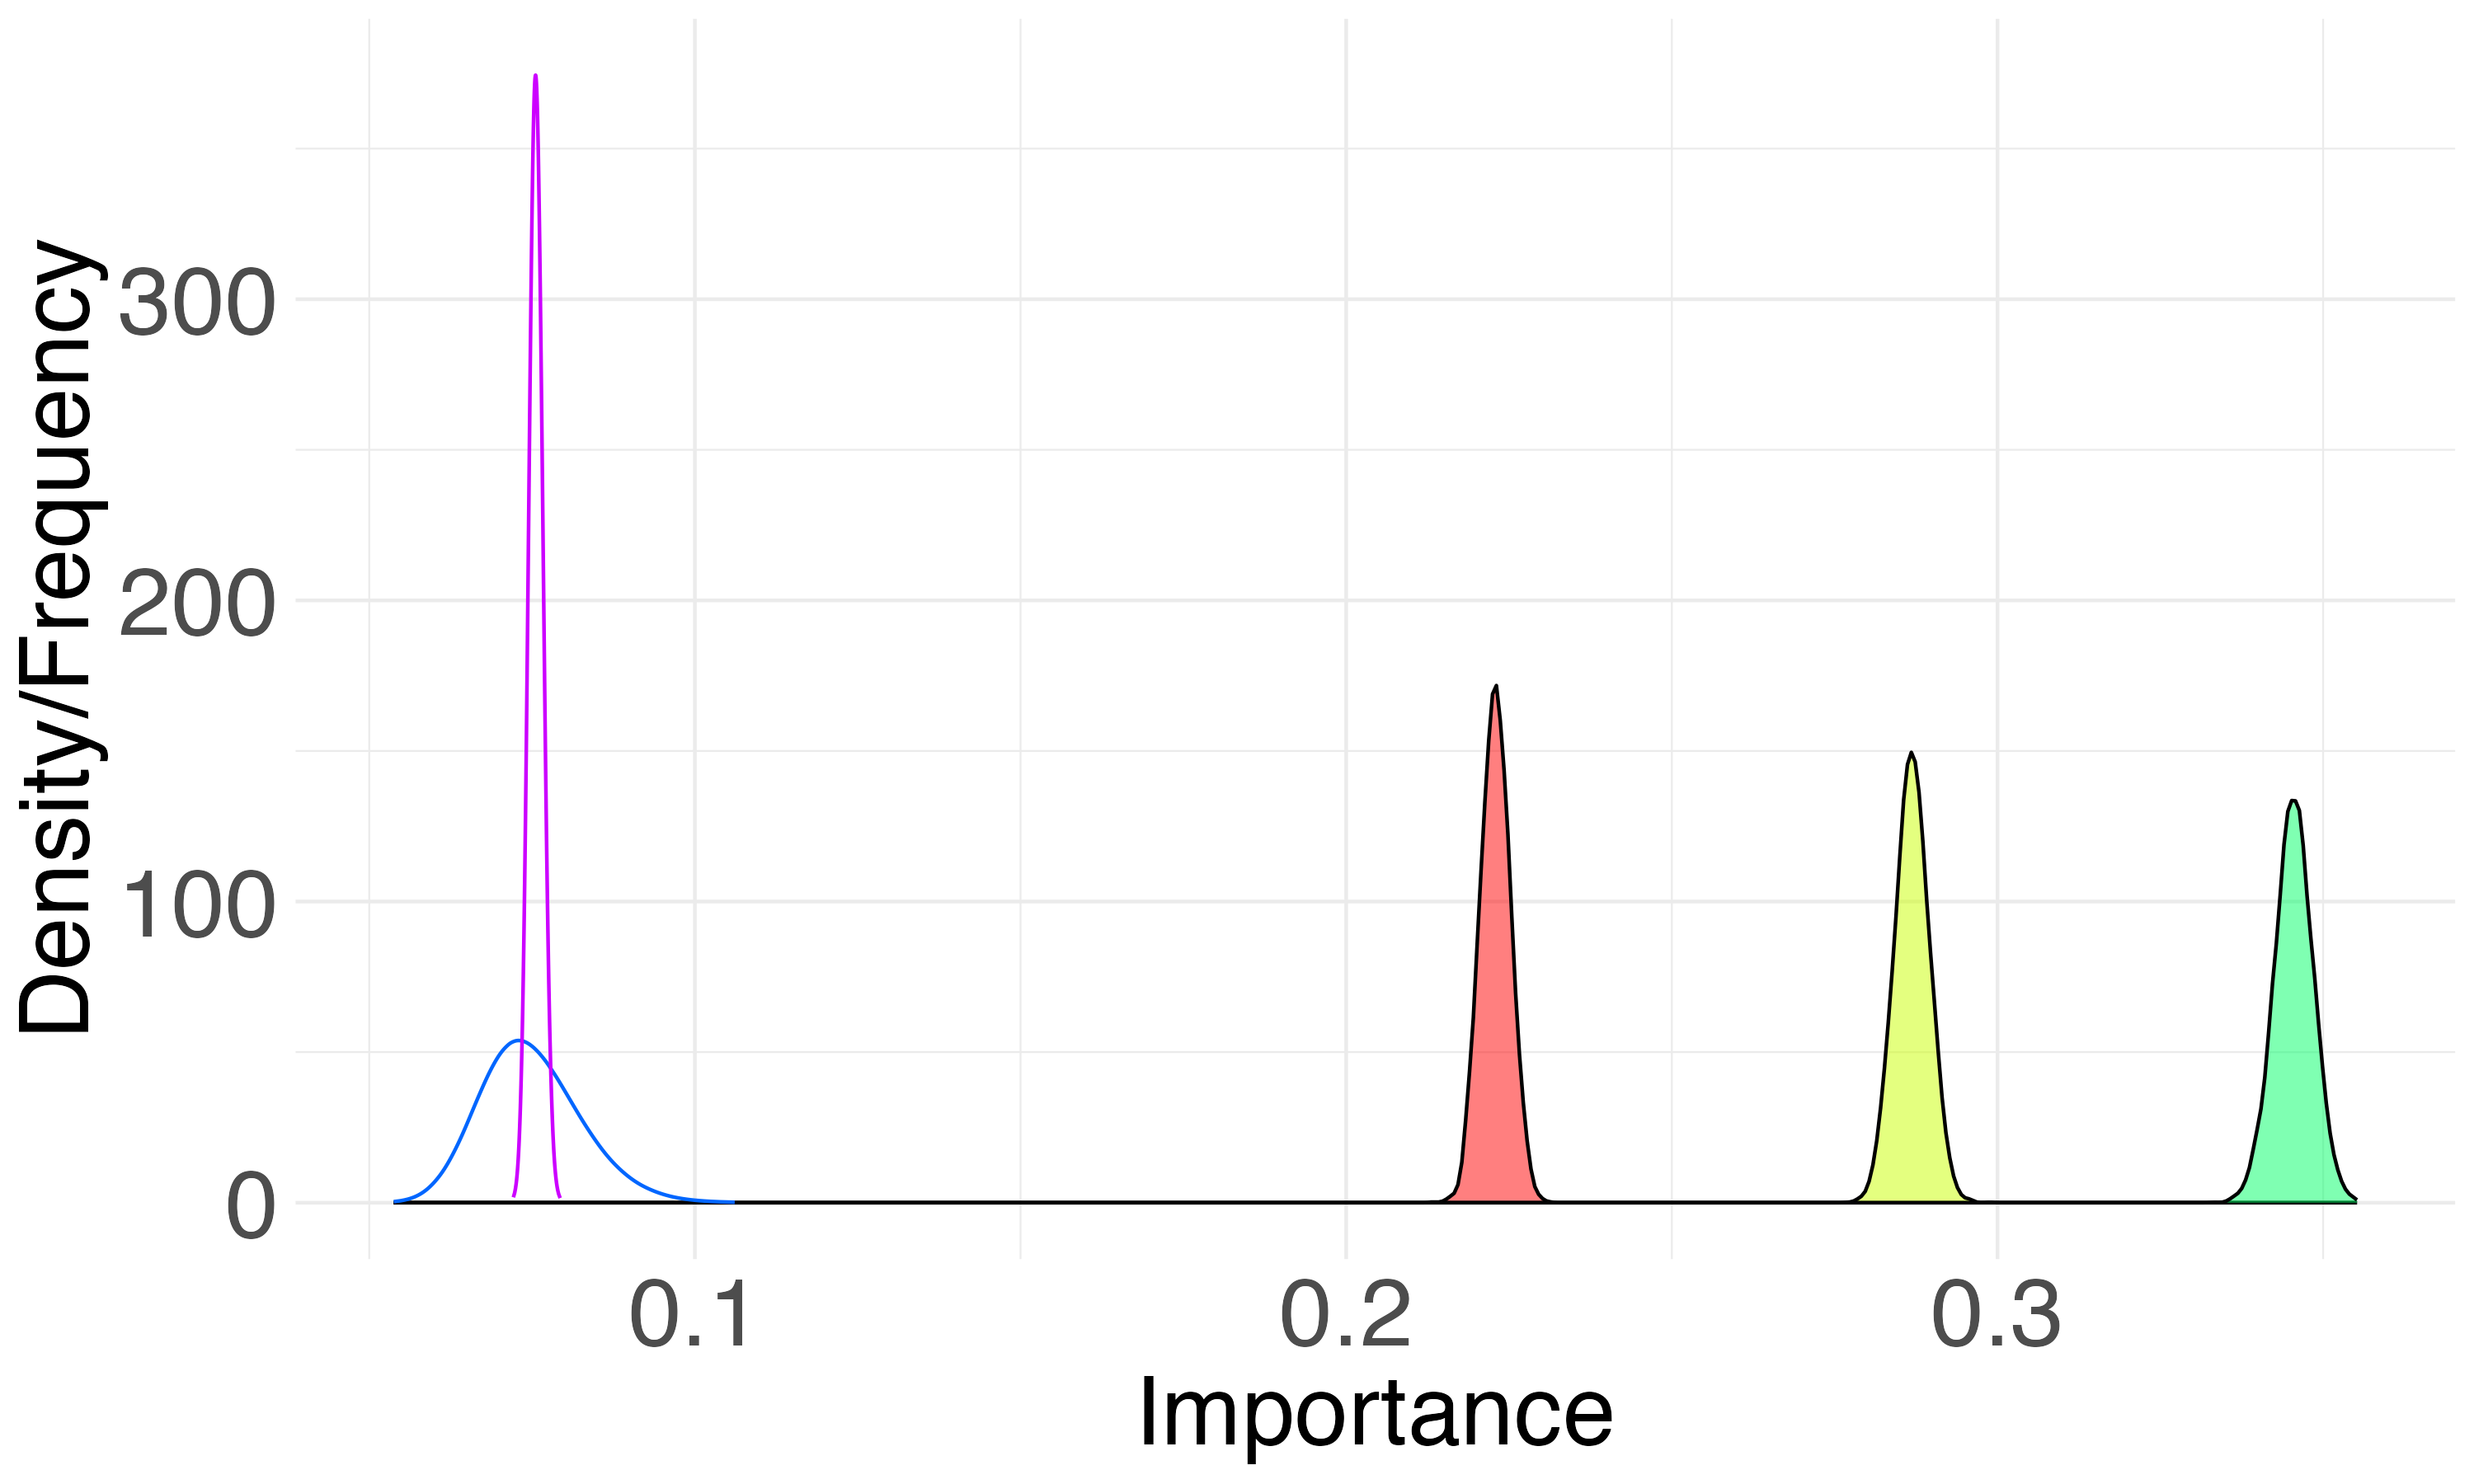
\includegraphics[width=0.5\linewidth]{Figures/Posterior Marginal/Posterior importance, cov=medium.png}
    \label{fig:posteriors_medium}
  }
  \subfloat[$\rho=0.9$]{
    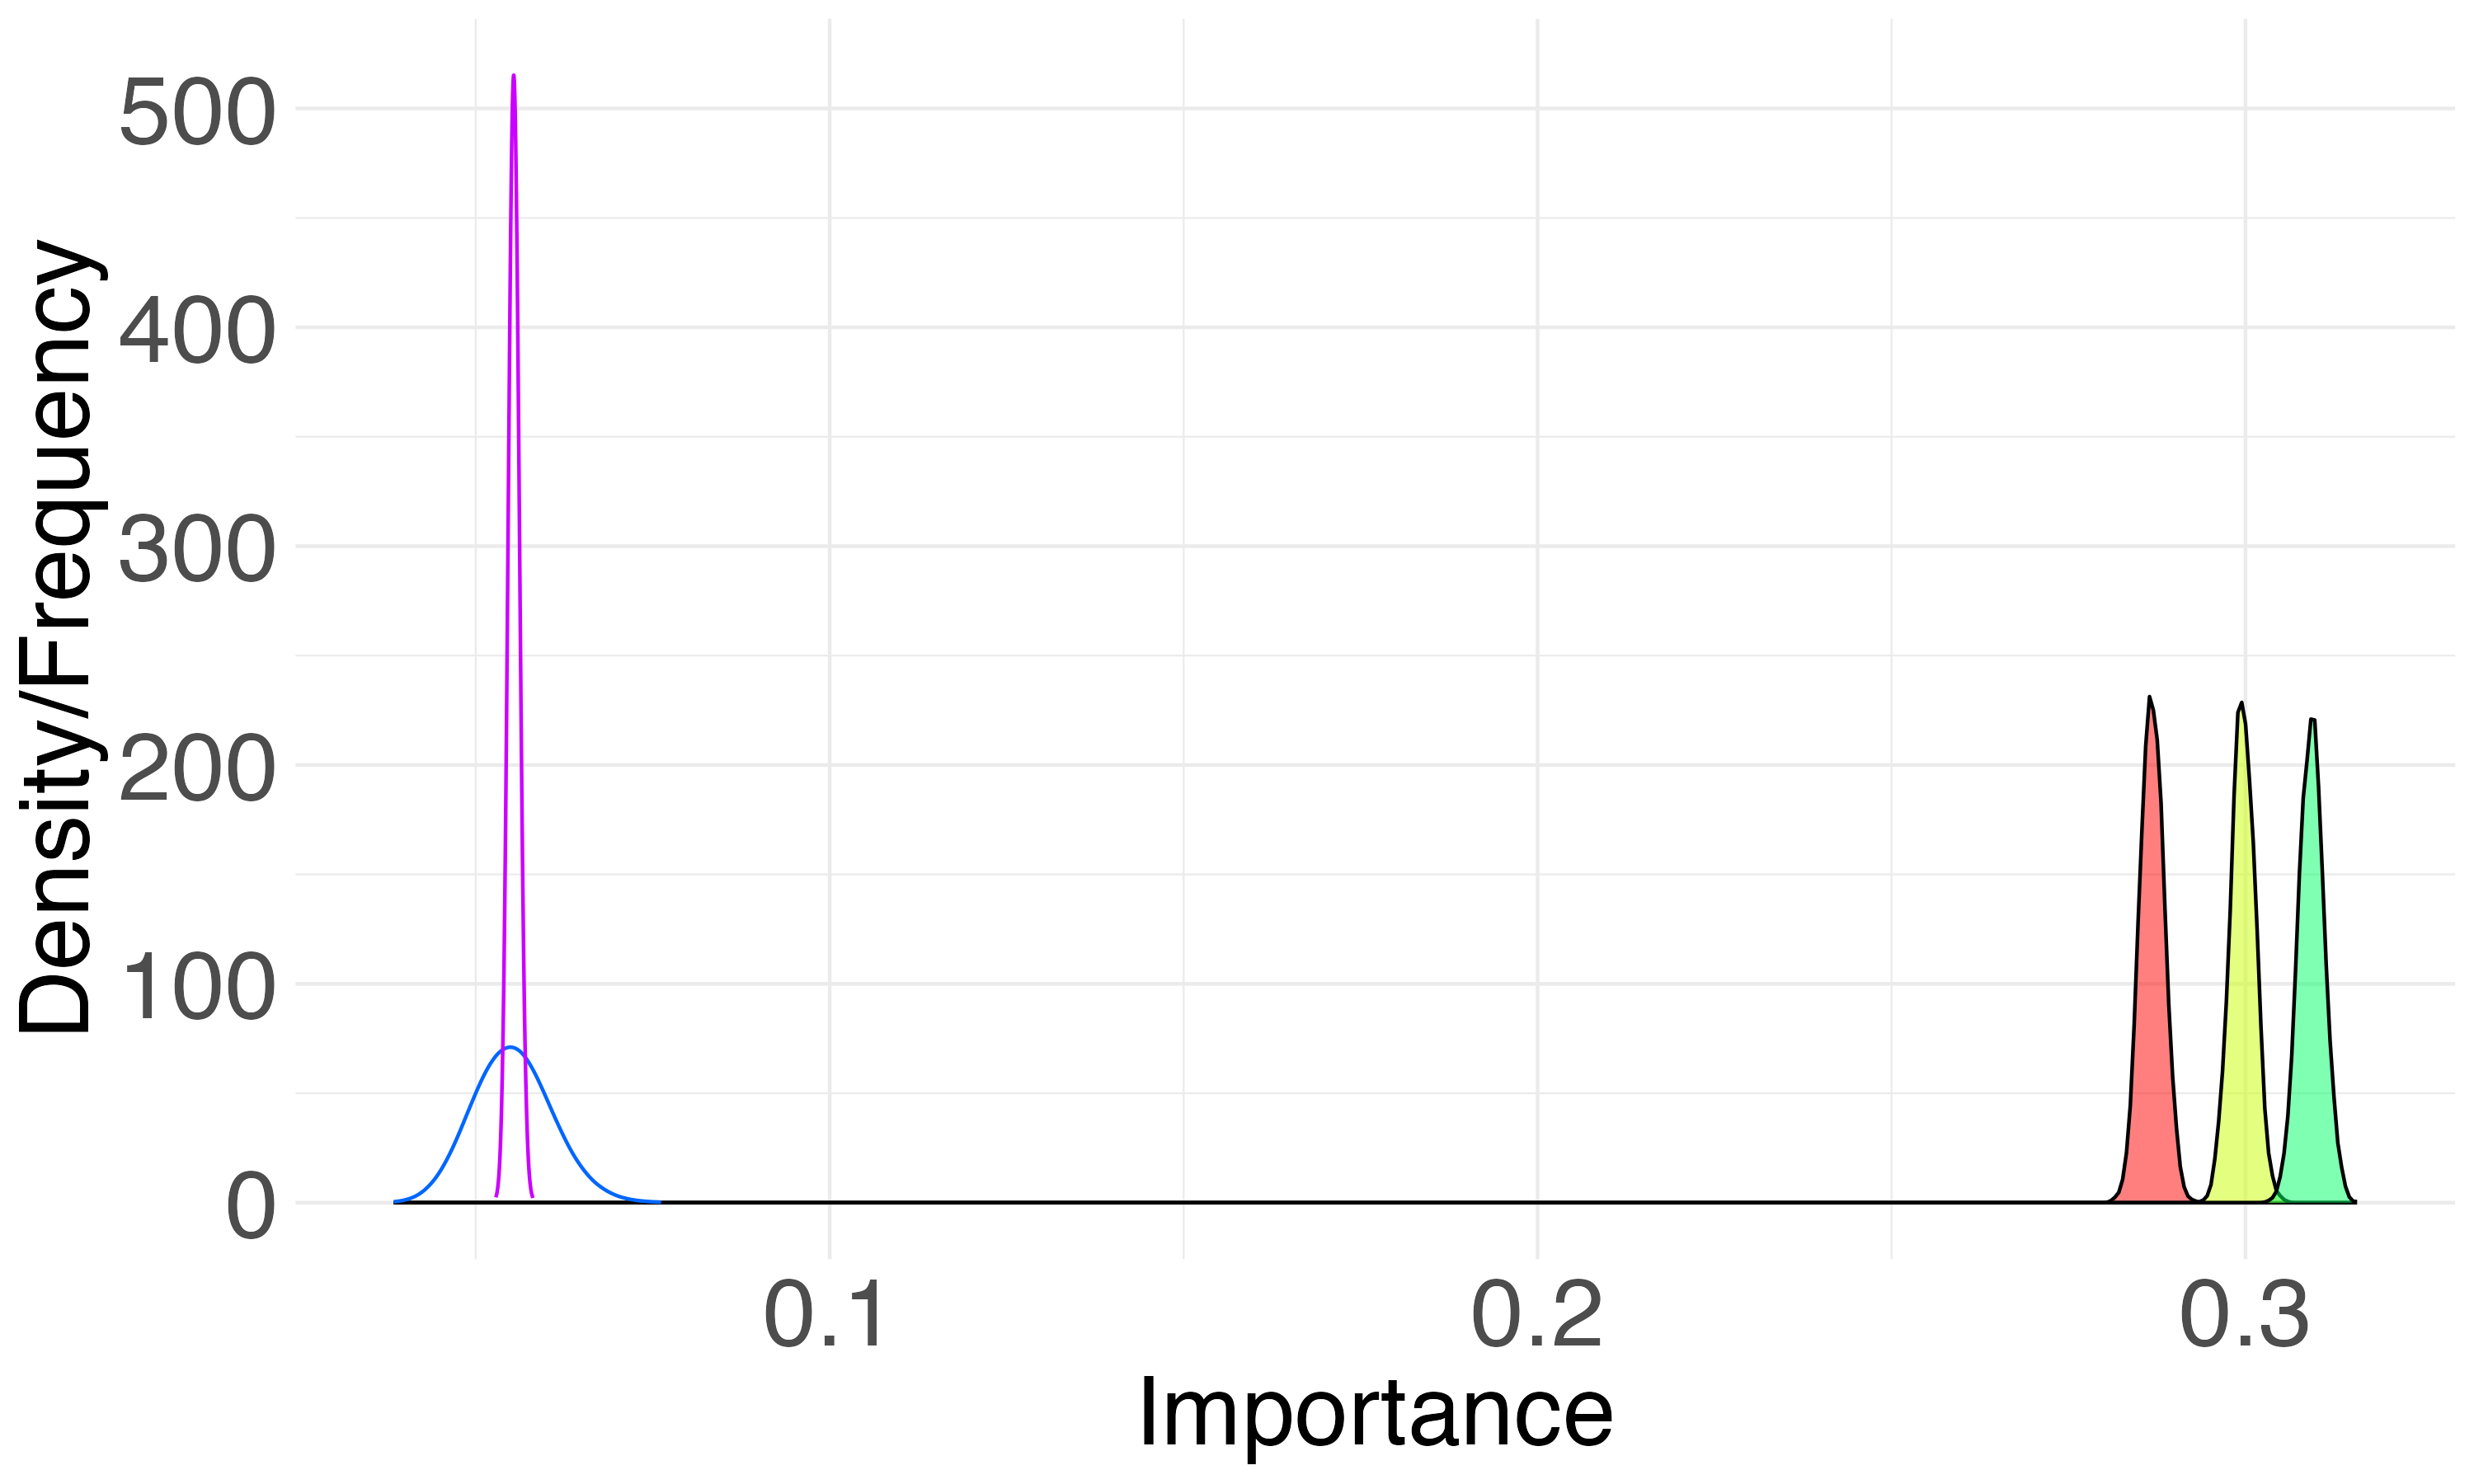
\includegraphics[width=0.5\linewidth]{Figures/Posterior Marginal/Posterior importance, cov=high.png}
    \label{fig:posteriors_high}
  }

  \caption{Posterior distributions for fixed effects and posterior marginal distributions for random effects from the BVI method on four randomly simulated datasets with different correlation values between the fixed effects. The blue and purple densities are the marginal posteriors for $\hat{\sigma}^2_{\alpha}$ and $\hat{\sigma}^2_{\varepsilon}$ respectively, whereas the red, yellow and green densities are the sampled posteriors for $X_1, X_2$ and $X_3$ respectively. The vertical lines in (a) represent the theoretically correct relative importances.}
  \label{fig:posterior_distributions}
\end{figure}
\newpage
\subsection{Posterior $R^2$ distributions}
From the above discussed posterior distributions, the posterior distributions of marginal (\Cref{fig:marginal_R2}) and conditional (\Cref{fig:conditional_R2}) variance explained, \textit{i.e.} $R^2$, can also be obtained.
As was the case for the posterior distributions of fixed and random effects, the $R^2$ distributions are also desired to possess a degree of stochasticity causing them to deviate moderately from the theoretical value.
We notice that in the uncorrelated case the $R^2$ is evenly distributed around the theoretically expected variance explained. 
For $\rho=0.1$ and $\rho=0.9$ the distribution of $R^2$ seem to be a skewed to the right when comparing it to the theoretically expected value and the distribution for $\rho=0.5$ skewed to the left.
The width of the distributions seem to narrow as correlation levels increase, as a result of the decreasing width in the individual posterior distributions of random and fixed effects.
\newline
\newline
Moving on to the conditional $R^2$ (\Cref{fig:conditional_R2}), which are displayed on the same scale as the marginal $R^2$, it is obvious that these distributions are tighter than the marginal $R^2$ distributions.
The scale is arguably too large to be used to display the conditional $R^2$ when one sees how narrow they are, but we chose to do so because of the comparison to the marginal $R^2$.
To the contrary, for $\rho=0.1$ and $\rho=0.9$ the distributions are skewed to the right. 
The marginal and conditional $R^2$ for the same model will be closely related so one should expect to see the same behaviour in both, as we do.
\newline
\newline
The posterior distributions of $R^2$ reflect our expectations as they exhibit the same stochasticity as seen for the posterior distributions of fixed and random effects.
\begin{figure}[H]
  \centering
  % First row
  \subfloat{
    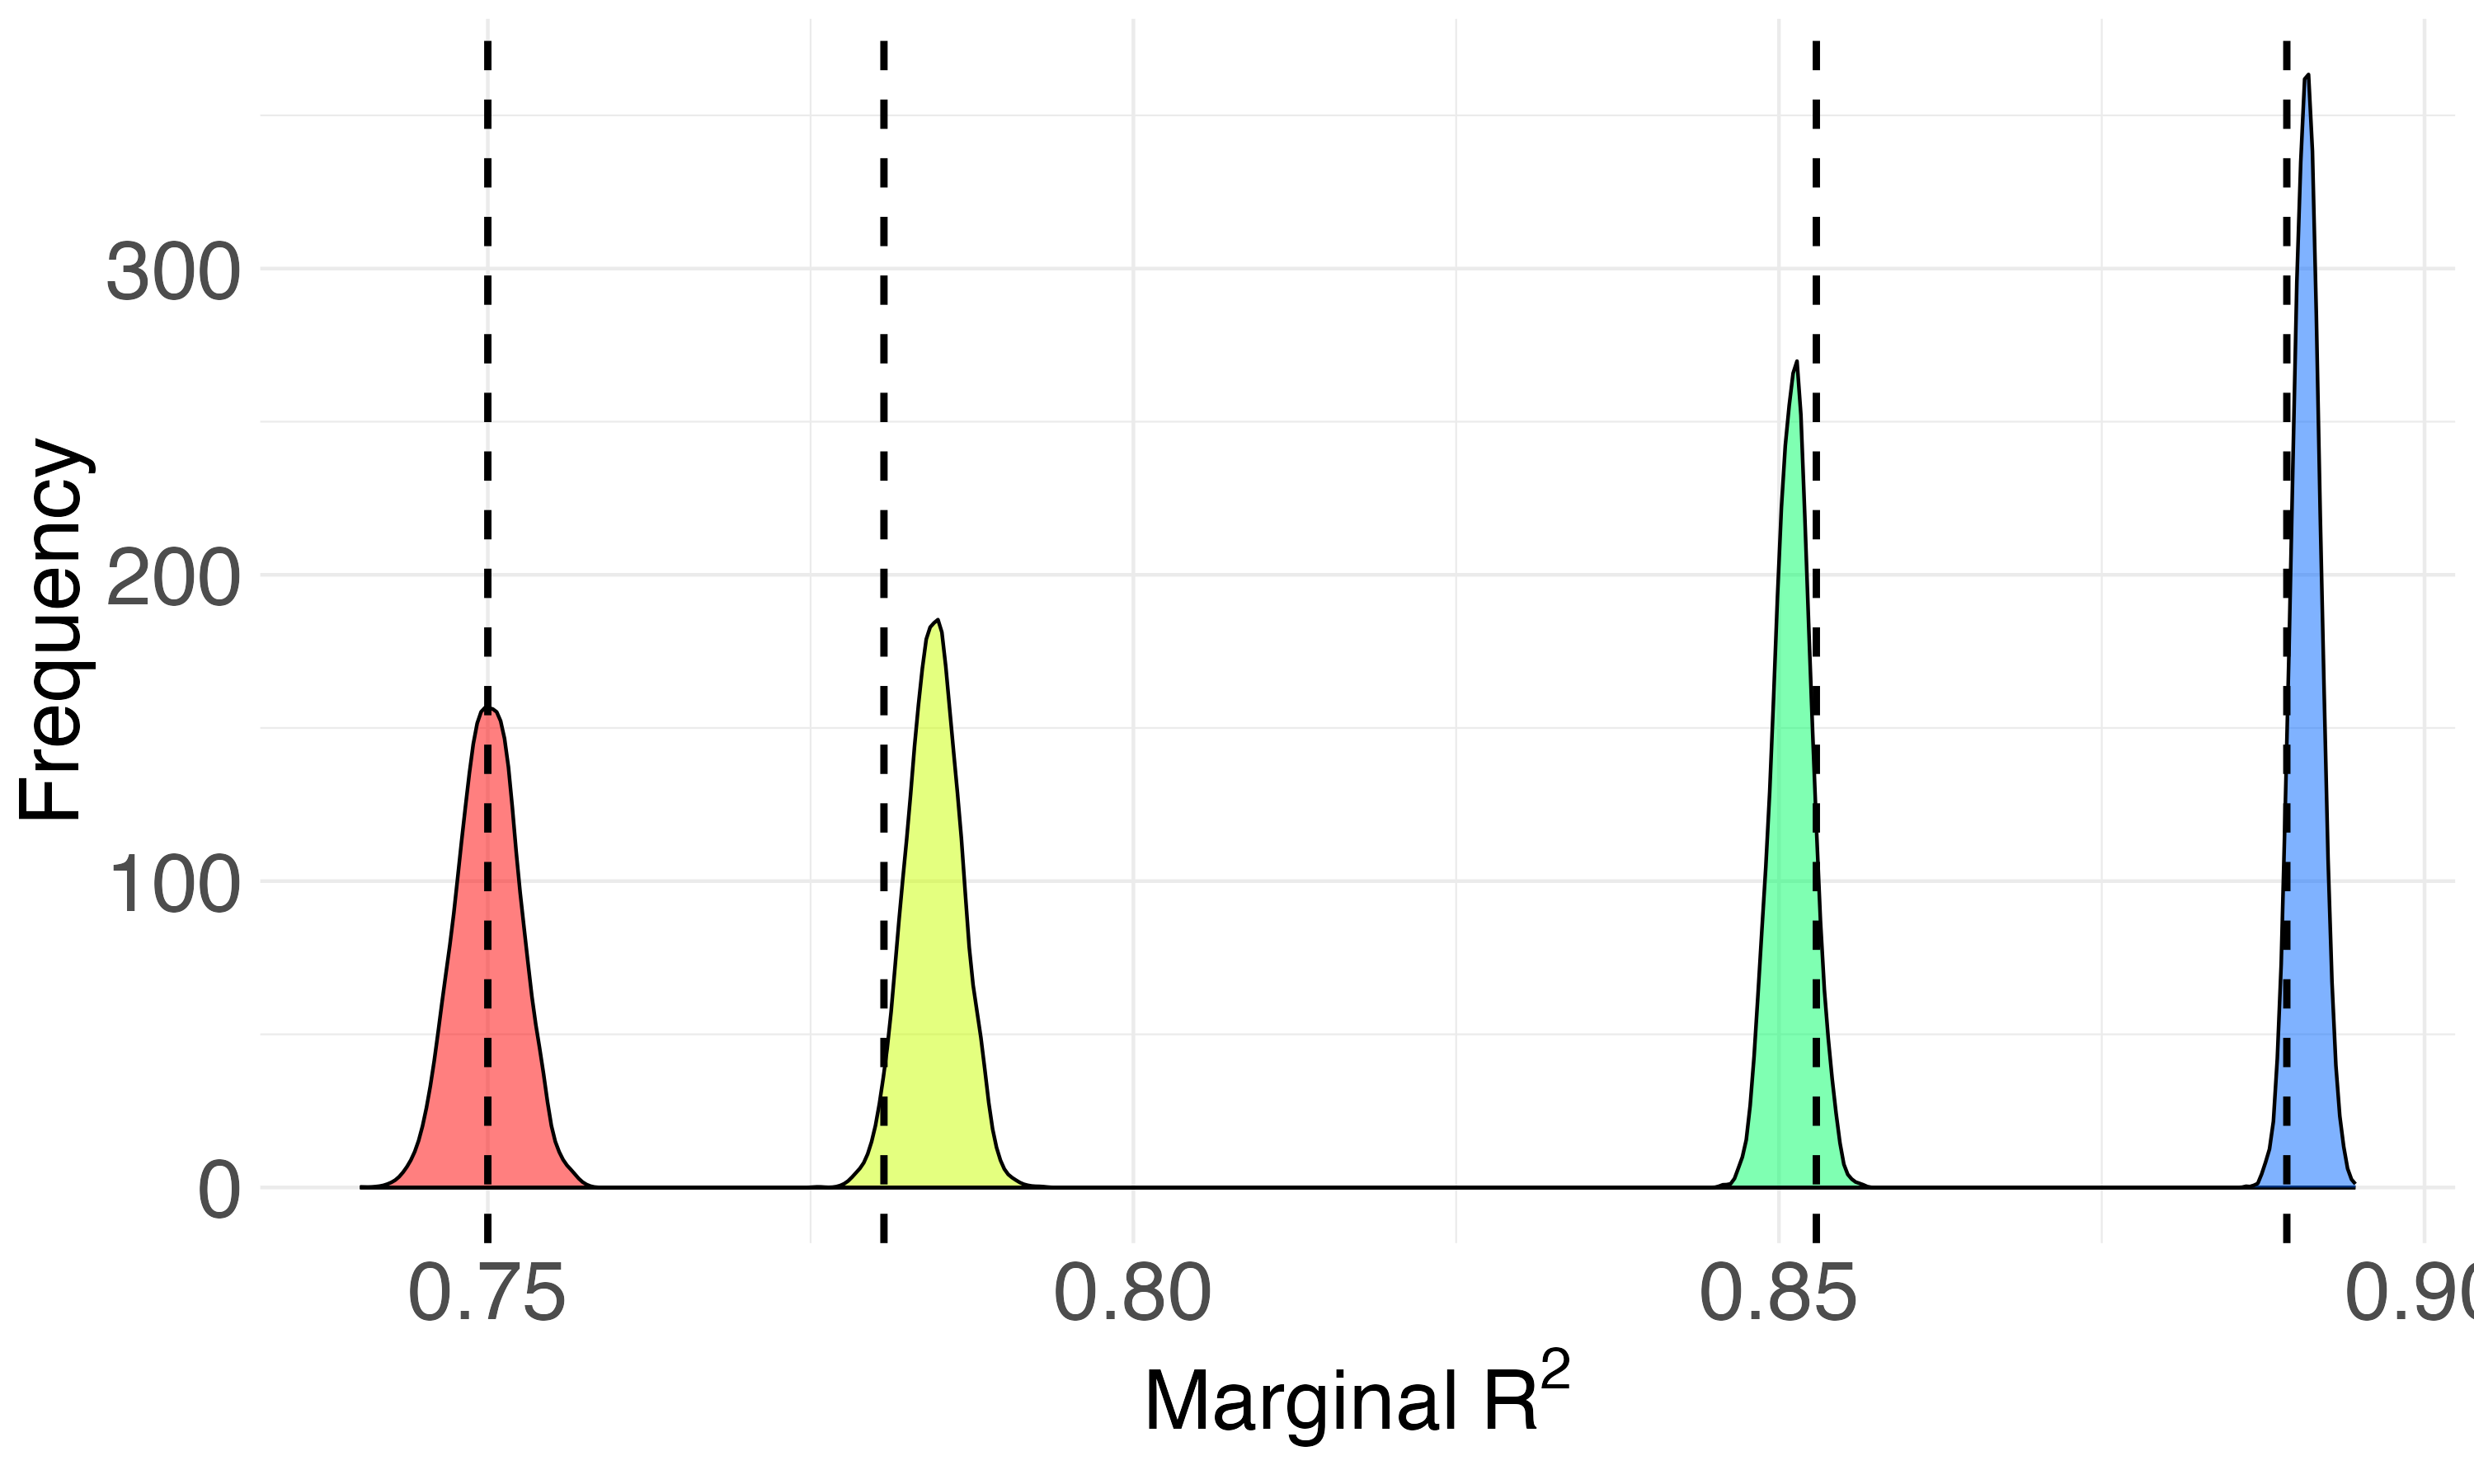
\includegraphics[width=0.7\linewidth]{Figures/R2/Marginal_R2.png}
    %\caption{Posterior marginal $R^2$ distribution calculated by the BVI method from the posterior distributions of fixed and random effects on four randomly simulated datasets with different correlation values $\rho$ between the fixed effects. The blue, green, red and purple distributions correspond to the posterior distribution of marginal $R^2$ for $\rho=0, \rho=0.1, \rho=0.5$ and $\rho=0.9$ respectively. The vertical lines represent the theoretically expected $R^2$ as presented in \Cref{table:1}.}
    \label{fig:marginal_R2}
  }
  \hfill
  \subfloat{
    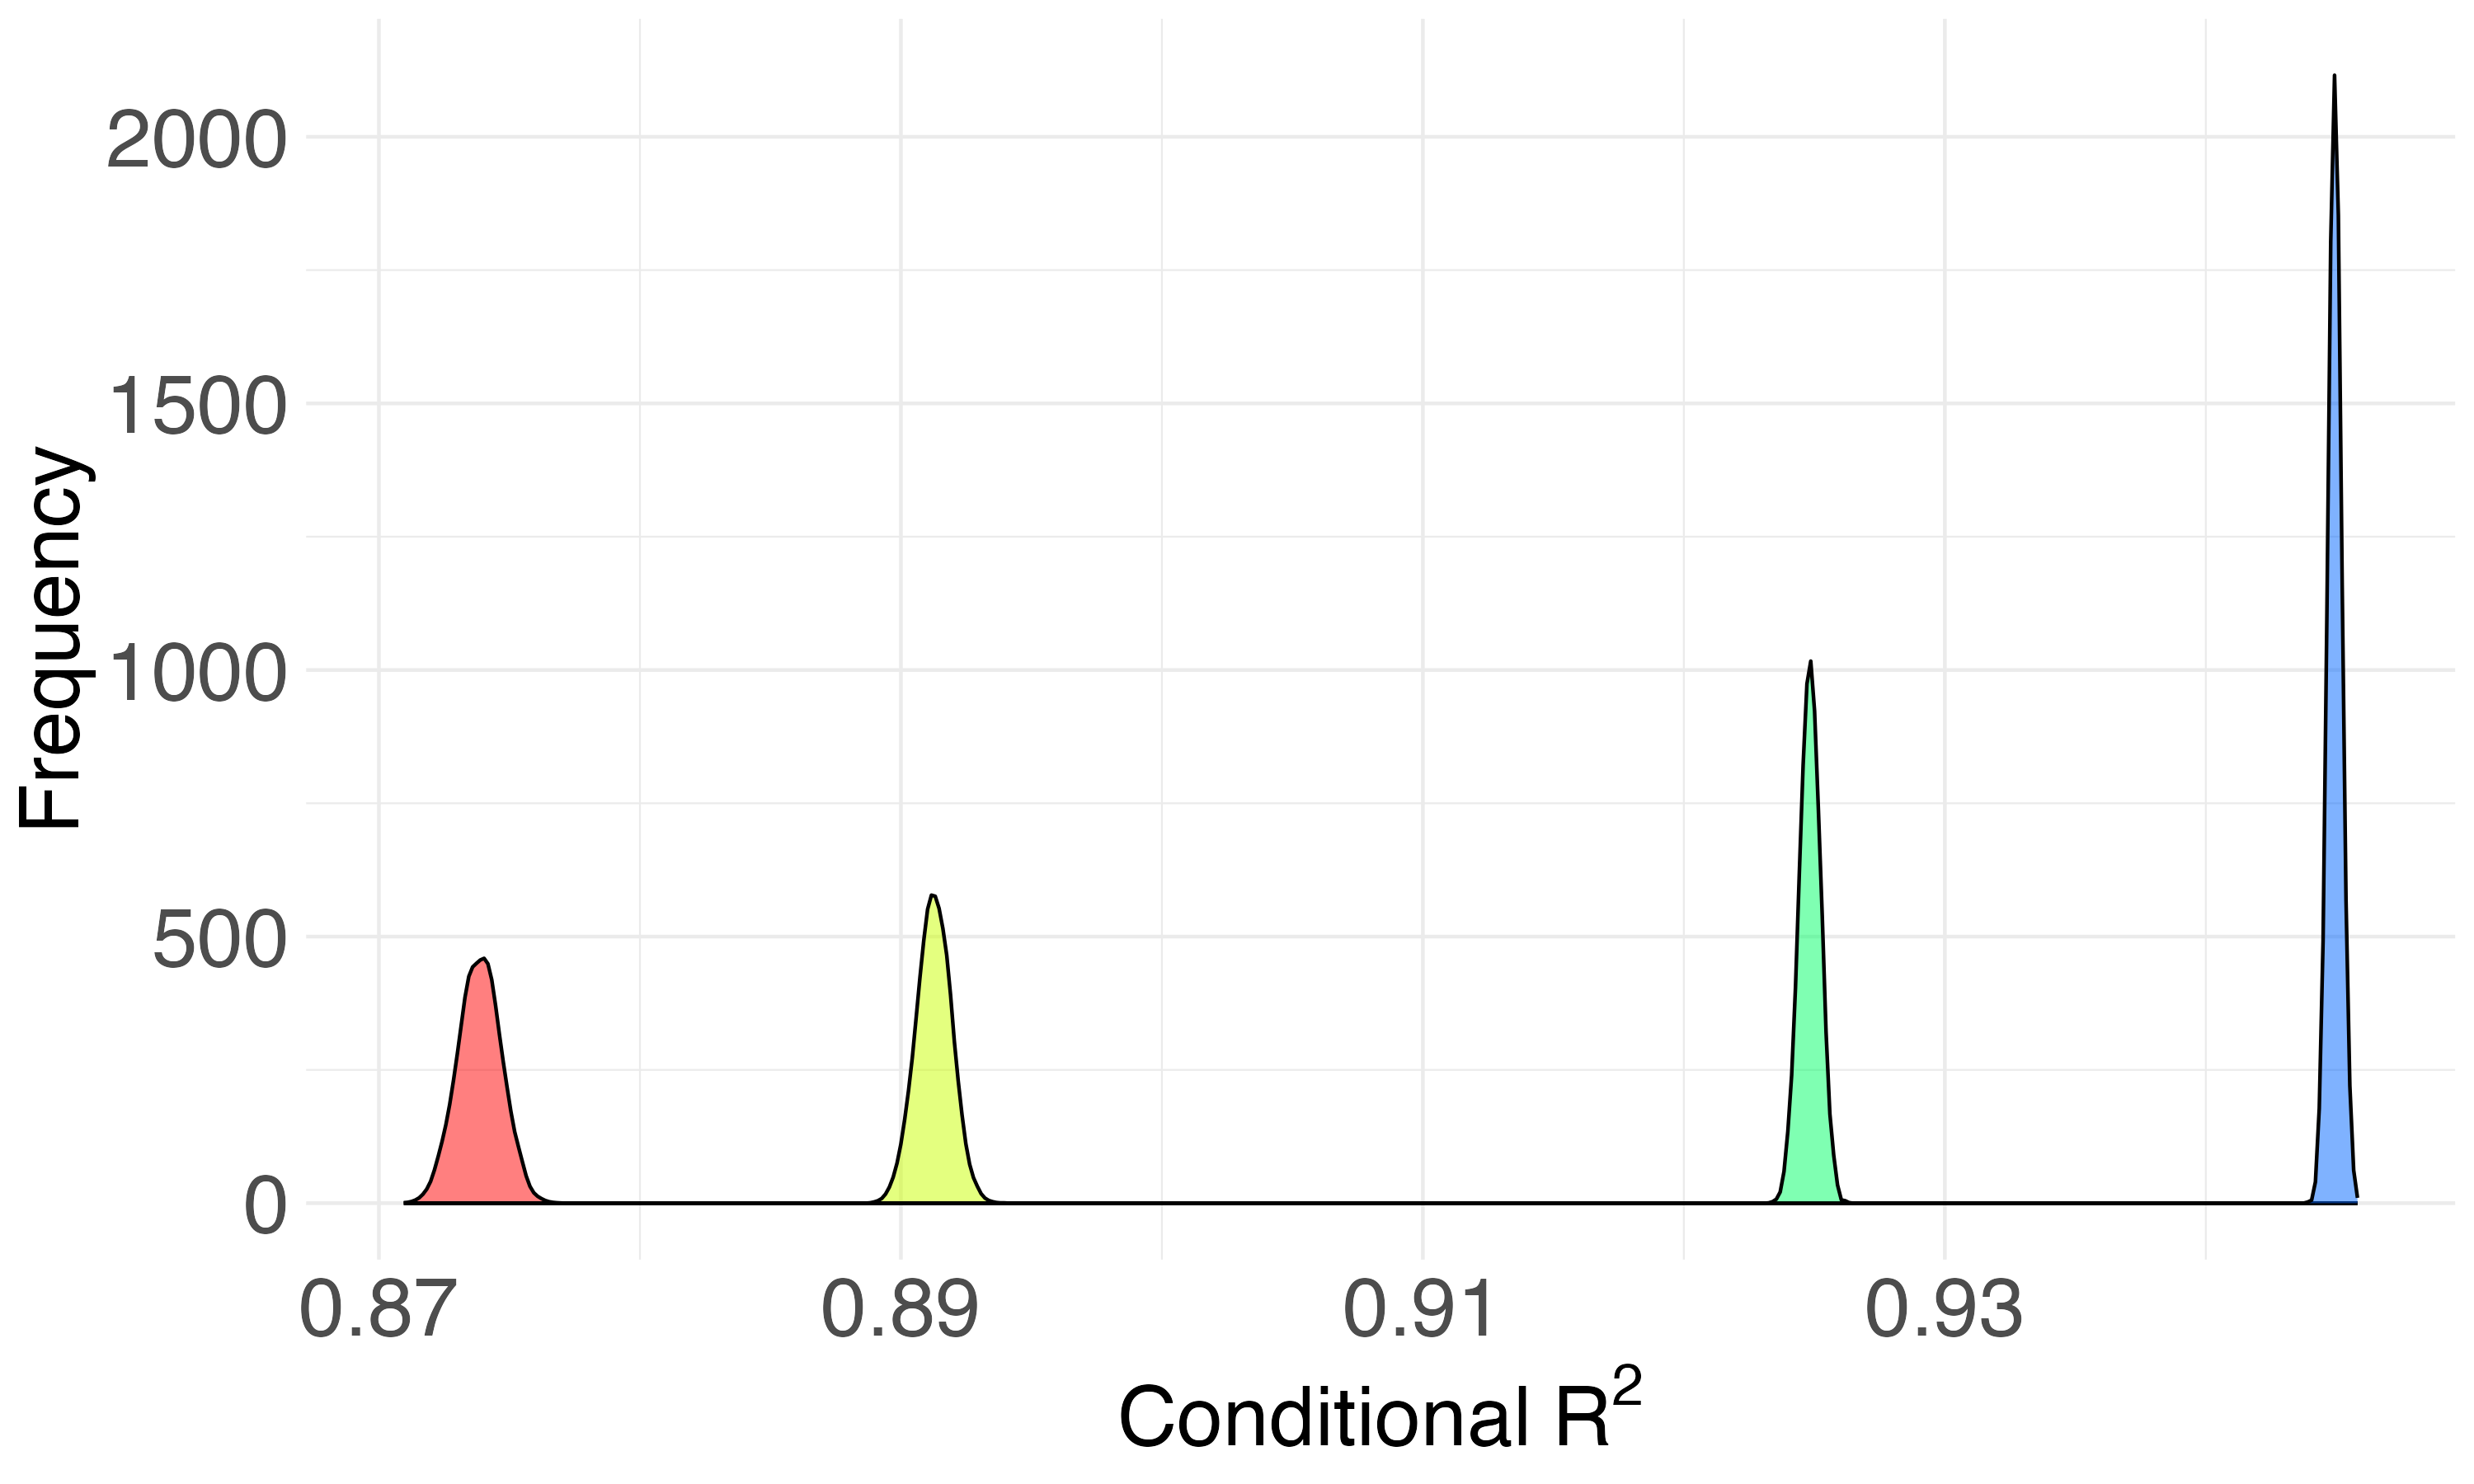
\includegraphics[width=0.7\linewidth]{Figures/R2/Conditional_R2.png}
    %\caption{Posterior conditional $R^2$ distribution calculated by the BVI method from the posterior distributions of fixed and random effects on four randomly simulated datasets with different correlation values $\rho$ between the fixed effects. The blue, green, red and purple distributions correspond to the posterior distribution of conditional $R^2$ for $\rho=0, \rho=0.1, \rho=0.5$ and $\rho=0.9$ respectively. The vertical lines represent the theoretically expected $R^2$ as presented in \Cref{table:1}.}
    \label{fig:conditional_R2}
  }
  \caption{Posterior $R^2$ distribution calculated by the BVI method from the posterior distributions of fixed and random effects on four randomly simulated datasets with different correlation values $\rho$ between the fixed effects. The red, yellow, green and blue distributions correspond to the posterior distribution of $R^2$ for $\rho=0, \rho=0.1, \rho=0.5$ and $\rho=0.9$ respectively. The theoretical values can be found in \Cref{table:1} and are shown as vertical lines.}
  \label{fig:R2}
\end{figure}



